% Options for packages loaded elsewhere
\PassOptionsToPackage{unicode}{hyperref}
\PassOptionsToPackage{hyphens}{url}
%
\documentclass[
]{article}
\usepackage{amsmath,amssymb}
\usepackage{iftex}
\ifPDFTeX
  \usepackage[T1]{fontenc}
  \usepackage[utf8]{inputenc}
  \usepackage{textcomp} % provide euro and other symbols
\else % if luatex or xetex
  \usepackage{unicode-math} % this also loads fontspec
  \defaultfontfeatures{Scale=MatchLowercase}
  \defaultfontfeatures[\rmfamily]{Ligatures=TeX,Scale=1}
\fi
\usepackage{lmodern}
\ifPDFTeX\else
  % xetex/luatex font selection
\fi
% Use upquote if available, for straight quotes in verbatim environments
\IfFileExists{upquote.sty}{\usepackage{upquote}}{}
\IfFileExists{microtype.sty}{% use microtype if available
  \usepackage[]{microtype}
  \UseMicrotypeSet[protrusion]{basicmath} % disable protrusion for tt fonts
}{}
\makeatletter
\@ifundefined{KOMAClassName}{% if non-KOMA class
  \IfFileExists{parskip.sty}{%
    \usepackage{parskip}
  }{% else
    \setlength{\parindent}{0pt}
    \setlength{\parskip}{6pt plus 2pt minus 1pt}}
}{% if KOMA class
  \KOMAoptions{parskip=half}}
\makeatother
\usepackage{xcolor}
\usepackage[margin=1in]{geometry}
\usepackage{color}
\usepackage{fancyvrb}
\newcommand{\VerbBar}{|}
\newcommand{\VERB}{\Verb[commandchars=\\\{\}]}
\DefineVerbatimEnvironment{Highlighting}{Verbatim}{commandchars=\\\{\}}
% Add ',fontsize=\small' for more characters per line
\usepackage{framed}
\definecolor{shadecolor}{RGB}{248,248,248}
\newenvironment{Shaded}{\begin{snugshade}}{\end{snugshade}}
\newcommand{\AlertTok}[1]{\textcolor[rgb]{0.94,0.16,0.16}{#1}}
\newcommand{\AnnotationTok}[1]{\textcolor[rgb]{0.56,0.35,0.01}{\textbf{\textit{#1}}}}
\newcommand{\AttributeTok}[1]{\textcolor[rgb]{0.13,0.29,0.53}{#1}}
\newcommand{\BaseNTok}[1]{\textcolor[rgb]{0.00,0.00,0.81}{#1}}
\newcommand{\BuiltInTok}[1]{#1}
\newcommand{\CharTok}[1]{\textcolor[rgb]{0.31,0.60,0.02}{#1}}
\newcommand{\CommentTok}[1]{\textcolor[rgb]{0.56,0.35,0.01}{\textit{#1}}}
\newcommand{\CommentVarTok}[1]{\textcolor[rgb]{0.56,0.35,0.01}{\textbf{\textit{#1}}}}
\newcommand{\ConstantTok}[1]{\textcolor[rgb]{0.56,0.35,0.01}{#1}}
\newcommand{\ControlFlowTok}[1]{\textcolor[rgb]{0.13,0.29,0.53}{\textbf{#1}}}
\newcommand{\DataTypeTok}[1]{\textcolor[rgb]{0.13,0.29,0.53}{#1}}
\newcommand{\DecValTok}[1]{\textcolor[rgb]{0.00,0.00,0.81}{#1}}
\newcommand{\DocumentationTok}[1]{\textcolor[rgb]{0.56,0.35,0.01}{\textbf{\textit{#1}}}}
\newcommand{\ErrorTok}[1]{\textcolor[rgb]{0.64,0.00,0.00}{\textbf{#1}}}
\newcommand{\ExtensionTok}[1]{#1}
\newcommand{\FloatTok}[1]{\textcolor[rgb]{0.00,0.00,0.81}{#1}}
\newcommand{\FunctionTok}[1]{\textcolor[rgb]{0.13,0.29,0.53}{\textbf{#1}}}
\newcommand{\ImportTok}[1]{#1}
\newcommand{\InformationTok}[1]{\textcolor[rgb]{0.56,0.35,0.01}{\textbf{\textit{#1}}}}
\newcommand{\KeywordTok}[1]{\textcolor[rgb]{0.13,0.29,0.53}{\textbf{#1}}}
\newcommand{\NormalTok}[1]{#1}
\newcommand{\OperatorTok}[1]{\textcolor[rgb]{0.81,0.36,0.00}{\textbf{#1}}}
\newcommand{\OtherTok}[1]{\textcolor[rgb]{0.56,0.35,0.01}{#1}}
\newcommand{\PreprocessorTok}[1]{\textcolor[rgb]{0.56,0.35,0.01}{\textit{#1}}}
\newcommand{\RegionMarkerTok}[1]{#1}
\newcommand{\SpecialCharTok}[1]{\textcolor[rgb]{0.81,0.36,0.00}{\textbf{#1}}}
\newcommand{\SpecialStringTok}[1]{\textcolor[rgb]{0.31,0.60,0.02}{#1}}
\newcommand{\StringTok}[1]{\textcolor[rgb]{0.31,0.60,0.02}{#1}}
\newcommand{\VariableTok}[1]{\textcolor[rgb]{0.00,0.00,0.00}{#1}}
\newcommand{\VerbatimStringTok}[1]{\textcolor[rgb]{0.31,0.60,0.02}{#1}}
\newcommand{\WarningTok}[1]{\textcolor[rgb]{0.56,0.35,0.01}{\textbf{\textit{#1}}}}
\usepackage{graphicx}
\makeatletter
\def\maxwidth{\ifdim\Gin@nat@width>\linewidth\linewidth\else\Gin@nat@width\fi}
\def\maxheight{\ifdim\Gin@nat@height>\textheight\textheight\else\Gin@nat@height\fi}
\makeatother
% Scale images if necessary, so that they will not overflow the page
% margins by default, and it is still possible to overwrite the defaults
% using explicit options in \includegraphics[width, height, ...]{}
\setkeys{Gin}{width=\maxwidth,height=\maxheight,keepaspectratio}
% Set default figure placement to htbp
\makeatletter
\def\fps@figure{htbp}
\makeatother
\setlength{\emergencystretch}{3em} % prevent overfull lines
\providecommand{\tightlist}{%
  \setlength{\itemsep}{0pt}\setlength{\parskip}{0pt}}
\setcounter{secnumdepth}{-\maxdimen} % remove section numbering
\ifLuaTeX
  \usepackage{selnolig}  % disable illegal ligatures
\fi
\IfFileExists{bookmark.sty}{\usepackage{bookmark}}{\usepackage{hyperref}}
\IfFileExists{xurl.sty}{\usepackage{xurl}}{} % add URL line breaks if available
\urlstyle{same}
\hypersetup{
  pdftitle={Regression Analysis on Car Specifications},
  pdfauthor={Luka Babić, Dominik Barukčić, Andrija Merlin, Ivan Skukan},
  hidelinks,
  pdfcreator={LaTeX via pandoc}}

\title{Regression Analysis on Car Specifications}
\author{Luka Babić, Dominik Barukčić, Andrija Merlin, Ivan Skukan}
\date{2024-01-11}

\begin{document}
\maketitle

\section{Uvod, motivacija i opis
problema}\label{uvod-motivacija-i-opis-problema}

U procesu kupovine novog automobila korisno je razmotriti njihove
specifikacije kako bi se donijela ˇsto objektivnija odluka o modelu koji
odgovara svim zahtjevima kupca. U tu su svrhu prikupljeni detaljni
podatci o modelima 22 proizvodaˇca automobila razliˇcitih cjenovnih
kategorija.

\section{Pitanje 1 - Snaga automobila ovisno o
pogonu}\label{pitanje-1---snaga-automobila-ovisno-o-pogonu}

\textbf{Je li snaga automobila s prednjim pogonom veća od automobila s
drugim vrstama pogona?}

\subsection{Uvod}\label{uvod}

U istraživanju odgovora na ovo pitanje analiziramo kako tip pogona
automobila utječe na njegovu snagu. Usredotočeni smo na usporedbu snage
između vozila s prednjim pogonom (FWD), zadnjim pogonom (RWD) i pogonom
na sve kotače (4WD). Korištenjem detaljnih podataka o automobilima,
primjenjujemo statističke metode za razumijevanje ovih razlika. Cilj nam
je pružiti dublji uvid u performanse automobila s obzirom na njihov tip
pogona.

\subsection{Učitavanje podataka}\label{uux10ditavanje-podataka}

Podaci o specifikacijama automobila učitavaju se iz CSV datoteke, pri
čemu se uklanjaju svi redovi s nedostajućim vrijednostima, osiguravajući
tako pouzdanost analize. Posebno se ističu atributi `drive.wheel' i
`horsepower', koji su ključni za naše istraživanje o odnosu između tipa
pogona automobila i njegove snage.

\begin{Shaded}
\begin{Highlighting}[]
\NormalTok{cardata }\OtherTok{=} \FunctionTok{read.csv}\NormalTok{(}\StringTok{\textquotesingle{}car\_specifications.csv\textquotesingle{}}\NormalTok{)}
\NormalTok{cardata }\OtherTok{=} \FunctionTok{na.omit}\NormalTok{(cardata)  }\CommentTok{\# Remove any rows with missing values}

\FunctionTok{head}\NormalTok{(cardata)}
\end{Highlighting}
\end{Shaded}

\begin{verbatim}
##         make aspiration num.of.doors  body.style drive.wheels engine.location
## 1 Alfa Romeo        std          two convertible          rwd           front
## 2 Alfa Romeo        std          two convertible          rwd           front
## 3 Alfa Romeo        std          two   hatchback          rwd           front
## 4       Audi        std         four       sedan          fwd           front
## 5       Audi        std         four       sedan          4wd           front
## 6       Audi        std          two       sedan          fwd           front
##   wheel.base length width height curb.weight engine.type num.of.cylinders
## 1      225.0  428.8 162.8  124.0        1156        dohc             four
## 2      225.0  428.8 162.8  124.0        1156        dohc             four
## 3      240.0  434.8 166.4  133.1        1280        ohcv              six
## 4      253.5  448.6 168.1  137.9        1060         ohc             four
## 5      252.5  448.6 168.7  137.9        1281         ohc             five
## 6      253.5  450.3 168.4  134.9        1137         ohc             five
##   engine.size fuel.system bore stroke compression.ratio horsepower peak.rpm
## 1        2130        mpfi 8.81   6.81               9.0        111     5000
## 2        2130        mpfi 8.81   6.81               9.0        111     5000
## 3        2491        mpfi 6.81   8.81               9.0        154     5000
## 4        1786        mpfi 8.10   8.64              10.0        102     5500
## 5        2229        mpfi 8.10   8.64               8.0        115     5500
## 6        2229        mpfi 8.10   8.64               8.5        110     5500
##   price city.L.100km highway.L.100km   fuel country continent
## 1 13495        11.19            8.70 petrol   Italy    Europe
## 2 16500        11.19            8.70 petrol   Italy    Europe
## 3 16500        12.37            9.04 petrol   Italy    Europe
## 4 13950         9.79            7.83 petrol Germany    Europe
## 5 17450        13.06           10.68 petrol Germany    Europe
## 6 15250        12.37            9.40 petrol Germany    Europe
\end{verbatim}

\subsection{Histogrami}\label{histogrami}

Generirajmo histograme koji vizualno prikazuju distribuciju snage motore
za svaku kategoriju pogona automobila - prednji (FWD), zadnji (RWD) i
pogon na sve kotače (4WD). Histogrami omogućuju vizualnu analizu razlika
u snazi između ovih triju kategorija.

\begin{Shaded}
\begin{Highlighting}[]
\CommentTok{\# Histograms of \textquotesingle{}horsepower\textquotesingle{} for each \textquotesingle{}drive.wheels\textquotesingle{} category}
\FunctionTok{hist}\NormalTok{(cardata}\SpecialCharTok{$}\NormalTok{horsepower[cardata}\SpecialCharTok{$}\NormalTok{drive.wheels}\SpecialCharTok{==}\StringTok{\textquotesingle{}fwd\textquotesingle{}}\NormalTok{], }\AttributeTok{main=}\StringTok{"Histogram of FWD Horsepower"}\NormalTok{, }\AttributeTok{xlab=}\StringTok{"Horsepower"}\NormalTok{)}
\end{Highlighting}
\end{Shaded}

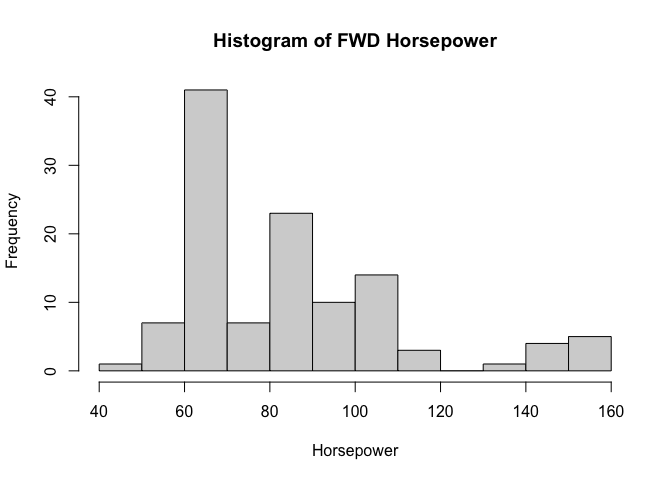
\includegraphics{AnabolicStatistics_files/figure-latex/unnamed-chunk-2-1.pdf}

\begin{Shaded}
\begin{Highlighting}[]
\FunctionTok{hist}\NormalTok{(cardata}\SpecialCharTok{$}\NormalTok{horsepower[cardata}\SpecialCharTok{$}\NormalTok{drive.wheels}\SpecialCharTok{==}\StringTok{\textquotesingle{}rwd\textquotesingle{}}\NormalTok{], }\AttributeTok{main=}\StringTok{"Histogram of RWD Horsepower"}\NormalTok{, }\AttributeTok{xlab=}\StringTok{"Horsepower"}\NormalTok{)}
\end{Highlighting}
\end{Shaded}

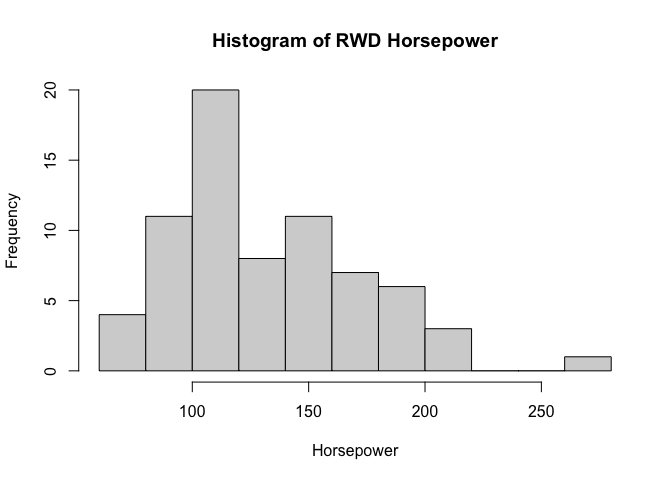
\includegraphics{AnabolicStatistics_files/figure-latex/unnamed-chunk-2-2.pdf}

\begin{Shaded}
\begin{Highlighting}[]
\FunctionTok{hist}\NormalTok{(cardata}\SpecialCharTok{$}\NormalTok{horsepower[cardata}\SpecialCharTok{$}\NormalTok{drive.wheels}\SpecialCharTok{==}\StringTok{\textquotesingle{}4wd\textquotesingle{}}\NormalTok{], }\AttributeTok{main=}\StringTok{"Histogram of 4WD Horsepower"}\NormalTok{, }\AttributeTok{xlab=}\StringTok{"Horsepower"}\NormalTok{)}
\end{Highlighting}
\end{Shaded}

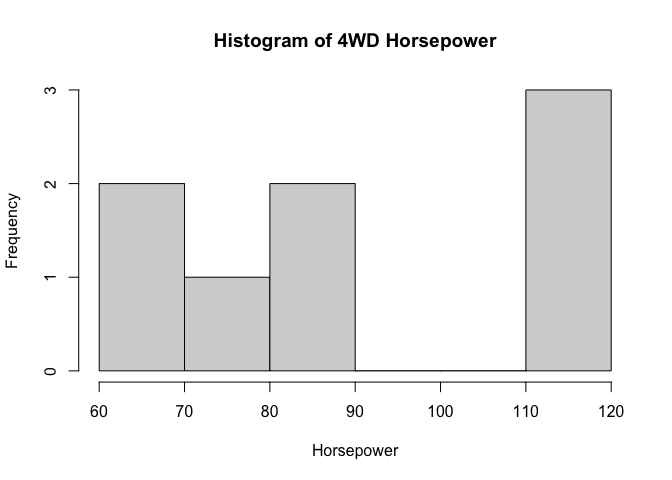
\includegraphics{AnabolicStatistics_files/figure-latex/unnamed-chunk-2-3.pdf}

Za 4WD vozila, histogram prikazuje da većina automobila s ovim tipom
pogona ima snagu koncentriranu oko manjih vrijednosti konjskih snaga (od
60 do 90 konjskih snaga), uz iznimku od 3 vozila sa snagom motora većom
od 110 konjskih snaga.

Za FWD vozila, histogram prikazuje vrlo visoku frekvenciju u nižem
rasponu snage, s vrhom oko 70 konjskih snaga. Distribucija je šira s
nižom maksimalnom učestalošću, što ukazuje na veći raspon snage motora
unutar ove kategorije, ali s tendencijom prema nižim vrijednostima
snage.

Za RWD vozila, histogram prikazuje distribuciju srednje koncentriranu
oko srednjeg raspona snage, s vrhom oko 150 konjskih snaga. Iako se
snaga proteže do viših vrijednosti, većina automobila s RWD pogonom ima
snagu unutar srednjeg raspona.

Ove distribucije ukazuju na različiti dizajn i cilj proizvođača za svaki
tip pogona. Na primjer, 4WD vozila su usmjerena na performanse i
sposobnost terenske vožnje, dok su FWD vozila više usmjerena na
ekonomičnost i praktičnost za svakodnevnu upotrebu. RWD vozila usmjerena
da budu sportski automobili koji zahtijevaju uravnoteženu raspodjelu
snage.

\subsection{Provjera normalnosti
podataka}\label{provjera-normalnosti-podataka}

Provodimo analizu normalnosti podataka za varijablu `horsepower' u
skladu s različitim vrstama pogona vozila. Koristimo QQ-plotove za
vizualizaciju distribucije `horsepower' za pogon na prednjim (FWD),
zadnjim (RWD) i četiri pogonska točka (4WD) te provodimo
Kolmogorov-Smirnov test (u biblioteci se zove lillie tj. Lilliefors
test) kako bismo provjerili normalnost podataka.

\begin{Shaded}
\begin{Highlighting}[]
\CommentTok{\# QQ{-}plots to check the normality of \textquotesingle{}horsepower\textquotesingle{} distribution for different drive types}
\CommentTok{\# QQ{-}plot for \textquotesingle{}horsepower\textquotesingle{} for front{-}wheel drive (fwd)}
\FunctionTok{qqnorm}\NormalTok{(cardata}\SpecialCharTok{$}\NormalTok{horsepower[cardata}\SpecialCharTok{$}\NormalTok{drive.wheels }\SpecialCharTok{==} \StringTok{\textquotesingle{}fwd\textquotesingle{}}\NormalTok{], }\AttributeTok{main =} \StringTok{"Q{-}Q Plot for FWD Horsepower"}\NormalTok{)}
\FunctionTok{qqline}\NormalTok{(cardata}\SpecialCharTok{$}\NormalTok{horsepower[cardata}\SpecialCharTok{$}\NormalTok{drive.wheels }\SpecialCharTok{==} \StringTok{\textquotesingle{}fwd\textquotesingle{}}\NormalTok{], }\AttributeTok{col =} \StringTok{"red"}\NormalTok{)}
\end{Highlighting}
\end{Shaded}

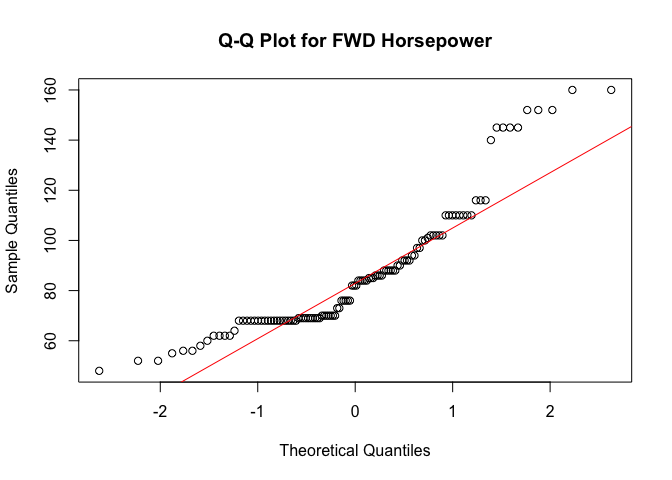
\includegraphics{AnabolicStatistics_files/figure-latex/unnamed-chunk-3-1.pdf}

\begin{Shaded}
\begin{Highlighting}[]
\CommentTok{\# QQ{-}plot for \textquotesingle{}horsepower\textquotesingle{} for rear{-}wheel drive (rwd)}
\FunctionTok{qqnorm}\NormalTok{(cardata}\SpecialCharTok{$}\NormalTok{horsepower[cardata}\SpecialCharTok{$}\NormalTok{drive.wheels }\SpecialCharTok{==} \StringTok{\textquotesingle{}rwd\textquotesingle{}}\NormalTok{], }\AttributeTok{main =} \StringTok{"Q{-}Q Plot for RWD Horsepower"}\NormalTok{)}
\FunctionTok{qqline}\NormalTok{(cardata}\SpecialCharTok{$}\NormalTok{horsepower[cardata}\SpecialCharTok{$}\NormalTok{drive.wheels }\SpecialCharTok{==} \StringTok{\textquotesingle{}rwd\textquotesingle{}}\NormalTok{], }\AttributeTok{col =} \StringTok{"red"}\NormalTok{)}
\end{Highlighting}
\end{Shaded}

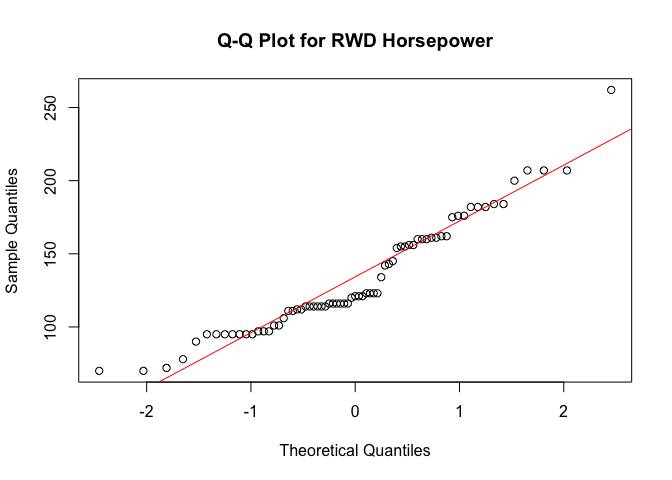
\includegraphics{AnabolicStatistics_files/figure-latex/unnamed-chunk-3-2.pdf}

\begin{Shaded}
\begin{Highlighting}[]
\CommentTok{\# QQ{-}plot for \textquotesingle{}horsepower\textquotesingle{} for four{-}wheel drive (4wd)}
\FunctionTok{qqnorm}\NormalTok{(cardata}\SpecialCharTok{$}\NormalTok{horsepower[cardata}\SpecialCharTok{$}\NormalTok{drive.wheels }\SpecialCharTok{==} \StringTok{\textquotesingle{}4wd\textquotesingle{}}\NormalTok{], }\AttributeTok{main =} \StringTok{"Q{-}Q Plot for 4WD Horsepower"}\NormalTok{)}
\FunctionTok{qqline}\NormalTok{(cardata}\SpecialCharTok{$}\NormalTok{horsepower[cardata}\SpecialCharTok{$}\NormalTok{drive.wheels }\SpecialCharTok{==} \StringTok{\textquotesingle{}4wd\textquotesingle{}}\NormalTok{], }\AttributeTok{col =} \StringTok{"red"}\NormalTok{)}
\end{Highlighting}
\end{Shaded}

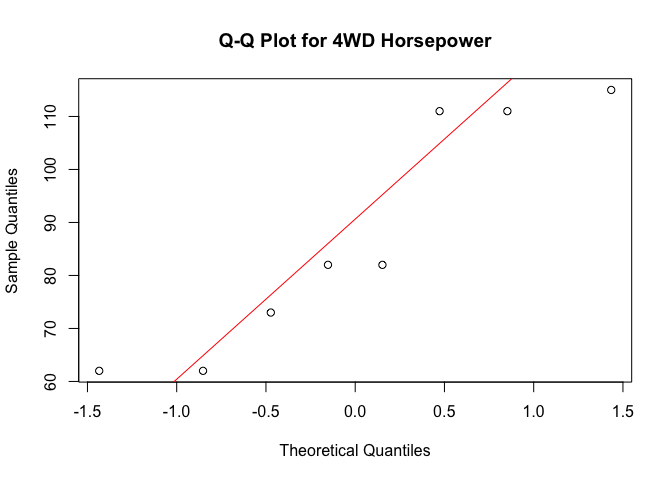
\includegraphics{AnabolicStatistics_files/figure-latex/unnamed-chunk-3-3.pdf}

\begin{Shaded}
\begin{Highlighting}[]
\CommentTok{\# Load package for Lilliefors (Kolmogorov{-}Smirnov) normality test}
\FunctionTok{require}\NormalTok{(nortest)}
\end{Highlighting}
\end{Shaded}

\begin{verbatim}
## Loading required package: nortest
\end{verbatim}

\begin{Shaded}
\begin{Highlighting}[]
\CommentTok{\# Normality tests for \textquotesingle{}horsepower\textquotesingle{} across different \textquotesingle{}drive.wheels\textquotesingle{} categories}
\FunctionTok{lillie.test}\NormalTok{(cardata}\SpecialCharTok{$}\NormalTok{horsepower)}
\FunctionTok{lillie.test}\NormalTok{(cardata}\SpecialCharTok{$}\NormalTok{horsepower[cardata}\SpecialCharTok{$}\NormalTok{drive.wheels }\SpecialCharTok{==} \StringTok{\textquotesingle{}fwd\textquotesingle{}}\NormalTok{])}
\FunctionTok{lillie.test}\NormalTok{(cardata}\SpecialCharTok{$}\NormalTok{horsepower[cardata}\SpecialCharTok{$}\NormalTok{drive.wheels }\SpecialCharTok{==} \StringTok{\textquotesingle{}rwd\textquotesingle{}}\NormalTok{])}
\FunctionTok{lillie.test}\NormalTok{(cardata}\SpecialCharTok{$}\NormalTok{horsepower[cardata}\SpecialCharTok{$}\NormalTok{drive.wheels }\SpecialCharTok{==} \StringTok{\textquotesingle{}4wd\textquotesingle{}}\NormalTok{])}
\end{Highlighting}
\end{Shaded}

\begin{verbatim}
## 
##  Lilliefors (Kolmogorov-Smirnov) normality test
## 
## data:  cardata$horsepower
## D = 0.12737, p-value = 3.598e-08
## 
## 
##  Lilliefors (Kolmogorov-Smirnov) normality test
## 
## data:  cardata$horsepower[cardata$drive.wheels == "fwd"]
## D = 0.16274, p-value = 5.212e-08
## 
## 
##  Lilliefors (Kolmogorov-Smirnov) normality test
## 
## data:  cardata$horsepower[cardata$drive.wheels == "rwd"]
## D = 0.19291, p-value = 6.33e-07
## 
## 
##  Lilliefors (Kolmogorov-Smirnov) normality test
## 
## data:  cardata$horsepower[cardata$drive.wheels == "4wd"]
## D = 0.23329, p-value = 0.2249
\end{verbatim}

Rezultati QQ-plotova ukazuju na odstupanja od pretpostavke normalnosti
za varijablu `horsepower' u svim kategorijama pogona vozila, pri čemu se
posebno izdvaja kategorija 4WD gdje se gotovo nijedan podatak ne
podudara s linearnom linijom na QQ-plotu.

Iz rezultata Kolmogorov-Smirnov testova za normalnost varijable
`horsepower' za različite kategorije pogona vozila (FWD, RWD i 4WD)
možemo izvući sljedeće zaključke:

\begin{enumerate}
\def\labelenumi{\arabic{enumi}.}
\tightlist
\item
  Za ukupni skup podataka, p-vrijednost testa je vrlo niska
  (p-vrijednost ≈ 3.598e-08), što ukazuje na to da distribucija
  `horsepower' varijable nije normalna.
\item
  Za kategoriju FWD, p-vrijednost je niska (p-vrijednost ≈ 5.212e-08),
  što ukazuje na to da distribucija `horsepower' za ovu kategoriju nije
  normalna.
\item
  Za kategoriju RWD, p-vrijednost je niska (p-vrijednost ≈ 6.33e-07),
  što ukazuje na to da distribucija `horsepower' za ovu kategoriju nije
  normalna.
\item
  Za kategoriju 4WD, p-vrijednost je relativno visoka (p-vrijednost ≈
  0.2249), što znači da nema dovoljno dokaza da distribucija
  `horsepower' za ovu kategoriju nije normalna.
\end{enumerate}

Na temelju ovih rezultata, zaključujemo da varijabla `horsepower' ne
ispunjava pretpostavku normalnosti distribucije u svim kategorijama
pogona vozila (FWD, RWD i 4WD). Posebno se ističe kategorija 4WD, gdje
nema dovoljno dokaza da distribucija `horsepower' nije normalna, ali i
dalje postoje znakovi odstupanja od normalnosti u ostalim kategorijama.

Unatoč padovima KS testova, uz naputak asistenta da QQ-plotovi ne
izgledaju ``loše'', dalje ćemo provesti Barlettov test i t-testove kao
da su podaci normalni.

\subsection{Barlettov test}\label{barlettov-test}

U ovom dijelu analize primjenjujemo Barlettov test kako bismo provjerili
homogenost varijanci varijable `horsepower' u različitim kategorijama
pogona vozila (FWD, RWD i 4WD). Također računamo varijance za
`horsepower' u svakoj od tih kategorija i prikazujemo distribuciju
`horsepower' putem boxplota kako bismo bolje razumjeli varijabilnost
podataka unutar svake kategorije.

\textbf{Uvjeti za Barlettov test} Kako bi proveli Barlettov test na
podacima, prvo moramo biti sigurni da dani podaci zadovoljavaju sljedeće
uvjete:

\begin{enumerate}
\def\labelenumi{\arabic{enumi}.}
\tightlist
\item
  Normalnost
\item
  Homogenost varijanci
\item
  Nezavisnost
\end{enumerate}

\textbf{Hipoteze}

\[H0:\ Nema\ statistički\ značajnih\ razlika\ u\ varijancama\ između\ grupa.
\\
H1:\ Postoje\ statistički\ značajne\ razlike\ u\ varijancama\ između\ grupa.\]

Uzimamo u obzir da su vozila u skupu podataka (retci) različita vozila i
pretpostavljamo da su podatci nezavisni. Ironično, uvjet testa je da su
varijance jednake, no bez obzira na taj zahtjev provodimo test kako bi
vidjeli ima li ikakve razlike u varijancama između grupa i kolike su te
razlike.

\begin{Shaded}
\begin{Highlighting}[]
\CommentTok{\# Bartlett\textquotesingle{}s test for homogeneity of variances across different \textquotesingle{}drive.wheels\textquotesingle{} categories}
\FunctionTok{bartlett.test}\NormalTok{(cardata}\SpecialCharTok{$}\NormalTok{horsepower }\SpecialCharTok{\textasciitilde{}}\NormalTok{ cardata}\SpecialCharTok{$}\NormalTok{drive.wheels)}

\CommentTok{\# Variance calculations for \textquotesingle{}horsepower\textquotesingle{} in each \textquotesingle{}drive.wheels\textquotesingle{} category}
\FunctionTok{var}\NormalTok{(cardata}\SpecialCharTok{$}\NormalTok{horsepower[cardata}\SpecialCharTok{$}\NormalTok{drive.wheels }\SpecialCharTok{==} \StringTok{\textquotesingle{}fwd\textquotesingle{}}\NormalTok{])}
\FunctionTok{var}\NormalTok{(cardata}\SpecialCharTok{$}\NormalTok{horsepower[cardata}\SpecialCharTok{$}\NormalTok{drive.wheels }\SpecialCharTok{==} \StringTok{\textquotesingle{}rwd\textquotesingle{}}\NormalTok{])}
\FunctionTok{var}\NormalTok{(cardata}\SpecialCharTok{$}\NormalTok{horsepower[cardata}\SpecialCharTok{$}\NormalTok{drive.wheels }\SpecialCharTok{==} \StringTok{\textquotesingle{}4wd\textquotesingle{}}\NormalTok{])}

\CommentTok{\# Boxplot showing distribution of \textquotesingle{}horsepower\textquotesingle{} across \textquotesingle{}drive.wheels\textquotesingle{} categories}
\FunctionTok{boxplot}\NormalTok{(cardata}\SpecialCharTok{$}\NormalTok{horsepower }\SpecialCharTok{\textasciitilde{}}\NormalTok{ cardata}\SpecialCharTok{$}\NormalTok{drive.wheels, }\AttributeTok{main=}\StringTok{"Boxplot of Horsepower by Drive Wheels"}\NormalTok{, }\AttributeTok{xlab=}\StringTok{"Drive Wheels"}\NormalTok{, }\AttributeTok{ylab=}\StringTok{"Horsepower"}\NormalTok{, }\AttributeTok{col=}\StringTok{"cyan"}\NormalTok{)}
\end{Highlighting}
\end{Shaded}

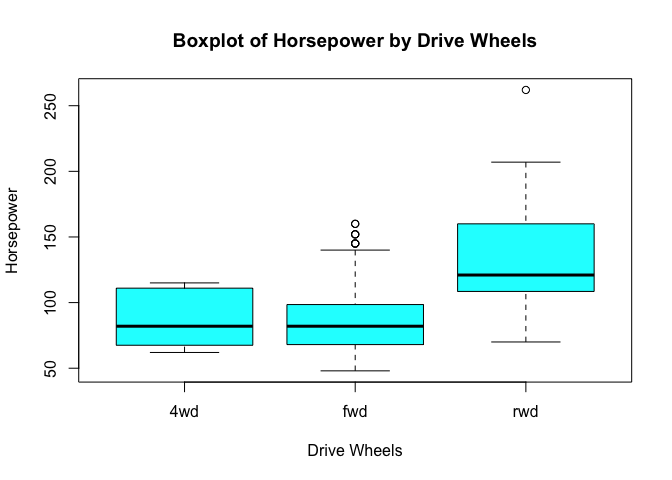
\includegraphics{AnabolicStatistics_files/figure-latex/unnamed-chunk-4-1.pdf}

\begin{verbatim}
## 
##  Bartlett test of homogeneity of variances
## 
## data:  cardata$horsepower by cardata$drive.wheels
## Bartlett's K-squared = 16.972, df = 2, p-value = 0.0002063
## 
## [1] 635.9978
## [1] 1481.587
## [1] 490.2143
\end{verbatim}

\textbf{Bartlettov test za homogenost varijanci je pružio značajne
rezultate:}

\begin{enumerate}
\def\labelenumi{\arabic{enumi}.}
\tightlist
\item
  Testna statistika Bartlett's K-squared iznosi 16.972.
\item
  Broj stupnjeva slobode (df) je 2 (broj kategorija koje se uspoređuju -
  1).
\item
  P-vrijednost (p-value) iznosi 0.0002063. S obzirom na p-vrijednost
  manju od uobičajene statističke značajnosti od 0.05, odbacujemo nultu
  hipotezu koja sugerira homogenost varijanci između grupa. Ovaj
  rezultat ukazuje na statistički značajne razlike u varijancama između
  barem dvije kategorije pogona vozila.
\end{enumerate}

\textbf{Na temelju izračunatih varijanci za varijablu `horsepower' u
različitim kategorijama pogona vozila, možemo izvući sljedeće
zaključke:}

\begin{enumerate}
\def\labelenumi{\arabic{enumi}.}
\tightlist
\item
  Vozila s prednjim pogonom (FWD) imaju relativno nisku varijancu snage
  motora (`horsepower') s vrijednošću od otprilike 635.9978. Ovo
  sugerira manju raznolikost snage motora unutar ove kategorije.
\item
  Vozila sa zadnjim pogonom (RWD) pokazuju znatno veću varijancu
  (`horsepower') koja iznosi približno 1481.587. To ukazuje na
  značajniju raspršenost snage motora među vozilima s zadnjim pogonom.
\item
  Kategorija vozila s pogonom na sva 4 kotača (4WD) ima umjerenu
  varijancu snage motora (`horsepower') koja iznosi otprilike 490.2143.
  Varijabilnost snage motora u ovoj kategoriji negdje je između FWD i
  RWD vozila.
\end{enumerate}

Razlike u varijancama sugeriraju da postoji znatna varijabilnost snage
motora između različitih kategorija pogona vozila, pri čemu RWD vozila
pokazuju najveću varijancu.

Boxplot prikazuje raspodjelu snage motora u tri različite kategorije
pogona vozila: pogon na sva četiri kotača (4WD), prednji pogon (FWD) i
stražnji pogon (RWD).

Pogon na sva četiri kotača (4WD): Kutija (interkvartilni raspon, IQR) je
relativno uska, što ukazuje na manju varijabilnost snage motora unutar
ove grupe. Medijan (označen crtom unutar kutije) iznosi oko 100 konjskih
snaga. Nema vidljivih izvanrednih vrijednosti, što sugerira da sva
vozila s pogonom na sva četiri kotača imaju snagu motora unutar
relativno konzistentnog raspona.

Prednji pogon (FWD): IQR je nešto veći nego kod 4WD-a, što ukazuje na
veću varijabilnost. Medijan snage motora nešto je niži nego kod 4WD-a, i
nalazi se blizu 100 konjskih snaga. Postoje neke izvanredne vrijednosti
ispod donjeg whiskera, što ukazuje da neka vozila s prednjim pogonom
imaju znatno manju snagu motora od ostalih.

Stražnji pogon (RWD): Ova kategorija ima najširi IQR, što sugerira širok
raspon vrijednosti snage motora. Medijan je puno viši u usporedbi s
druga dva, i nalazi se iznad 150 konjskih snaga. Postoji nekoliko
izvanrednih vrijednosti, i iznad i ispod kutije. Izvanredne vrijednosti
iznad gornjeg whiskera ukazuju da neka vozila s pogonom na stražnjim
kotačima imaju iznimno visoku snagu motora.

Općenito, vozila s pogonom na stražnjim kotačima obično imaju veću snagu
motora sa širim rasponom vrijednosti, dok vozila s pogonom na sva četiri
kotača imaju manju varijabilnost i vozila s prednjim pogonom obično
imaju manju snagu motora, s nekim iznimkama. Prisutnost izvanrednih
vrijednosti, posebno u kategoriji vozila s pogonom na stražnjim
kotačima, sugerira da postoje vozila s vrijednostima snage motora koje
se značajno razlikuju od tipičnog raspona vrijednosti unutar te
kategorije pogona na kotačima.

\subsection{Kruskal-Wallis test}\label{kruskal-wallis-test}

Kako bismo istražili moguće razlike u snazi motora (`horsepower') između
različitih kategorija pogona vozila, primijenili smo Kruskal-Wallis
test. Ovaj test omogućuje statističku provjeru postojanja značajnih
varijacija u snazi motora među tri različite kategorije pogonskih
točkica.

\textbf{Pretpostavke Kruskal-Wallis testa su sljedeće:}

\begin{enumerate}
\def\labelenumi{\arabic{enumi}.}
\tightlist
\item
  Grupe su nezavisne i slučajno uzorkovane.
\item
  Mjerenja su numerička ili ordinalna.
\end{enumerate}

Ovaj test je neosjetljiv na normalnost distribucije podataka i
homogenost varijanci te ga zato možemo provesti.

\textbf{Hipoteze:}
\[H0: Nema\ statistički\ značajnih\ razlika\ između\ grupa.\\H1: Postoji\ statistički\ značajna\ razlika\ između\ najmanje\ jedne\ od\ grupa\ u\ usporedbi.\]

\begin{Shaded}
\begin{Highlighting}[]
\CommentTok{\# Kruskal{-}Wallis test to check for differences in \textquotesingle{}horsepower\textquotesingle{} among the 3 drive wheel categories}
\FunctionTok{kruskal.test}\NormalTok{(horsepower }\SpecialCharTok{\textasciitilde{}}\NormalTok{ drive.wheels, }\AttributeTok{data =}\NormalTok{ cardata)}
\end{Highlighting}
\end{Shaded}

\begin{verbatim}
## 
##  Kruskal-Wallis rank sum test
## 
## data:  horsepower by drive.wheels
## Kruskal-Wallis chi-squared = 76.417, df = 2, p-value < 2.2e-16
\end{verbatim}

Test daje statističku vrijednost chi-kvadrat od 76,417 sa 2 stupnja
slobode. Izuzetno mala p-vrijednost, manja od 2.2e-16, ukazuje na
statistički značajnu razliku u raspodjeli snage motora među tri
kategorije pogonska. S obzirom na rezultate, možemo odbaciti nultu
hipotezu da je medijan snage motora isti za kategorije 4WD, FWD i RWD.
Drugim riječima, nije istina da nema statistički značajnih razlika
između grupa. Zaključak ovog testa podupire vizualne nalaze iz
boxplotova, gdje je uočeno da vozila sa stražnjim pogonom obično imaju
veću snagu motora, što sugerira da postoji razlika u snazi motora između
različitih vrsta pogona.

\subsection{T-test}\label{t-test}

Provodimo t-testove za usporedbu snage motora između različitih vrsta
pogona vozila. Uspoređujemo snagu motora između vozila s prednjim
pogonom (FWD), stražnjim pogonom (RWD) i pogonom na sva četiri kotača
(4WD). Cilj ovih testova je provjeriti postoje li statistički značajne
razlike u snazi motora između navedenih vrsta pogona vozila. Rezultati
testova pružit će nam bolji uvid u to kako različite vrste pogona mogu
utjecati na snagu motora u vozilima.

\textbf{T-test, koji se koristi za usporedbu srednjih vrijednosti dviju
grupa, ima tri glavne pretpostavke:}

\begin{enumerate}
\def\labelenumi{\arabic{enumi}.}
\tightlist
\item
  Normalnost distribucije
\item
  Homogenost varijanci
\item
  Nezavisnost uzoraka
\end{enumerate}

Budući da varijance nisu homogene, koristimo opciju var.equal = FALSE
pri provođenju testova.

\begin{Shaded}
\begin{Highlighting}[]
\CommentTok{\# T{-}test for \textquotesingle{}horsepower\textquotesingle{} between fwd and rwd}
\FunctionTok{t.test}\NormalTok{(cardata}\SpecialCharTok{$}\NormalTok{horsepower[cardata}\SpecialCharTok{$}\NormalTok{drive.wheels }\SpecialCharTok{==} \StringTok{\textquotesingle{}fwd\textquotesingle{}}\NormalTok{], }
\NormalTok{       cardata}\SpecialCharTok{$}\NormalTok{horsepower[cardata}\SpecialCharTok{$}\NormalTok{drive.wheels }\SpecialCharTok{==} \StringTok{\textquotesingle{}rwd\textquotesingle{}}\NormalTok{], }\AttributeTok{var.equal =} \ConstantTok{FALSE}\NormalTok{)}

\CommentTok{\# T{-}test for \textquotesingle{}horsepower\textquotesingle{} between rwd and 4wd}
\FunctionTok{t.test}\NormalTok{(cardata}\SpecialCharTok{$}\NormalTok{horsepower[cardata}\SpecialCharTok{$}\NormalTok{drive.wheels }\SpecialCharTok{==} \StringTok{\textquotesingle{}rwd\textquotesingle{}}\NormalTok{], }
\NormalTok{       cardata}\SpecialCharTok{$}\NormalTok{horsepower[cardata}\SpecialCharTok{$}\NormalTok{drive.wheels }\SpecialCharTok{==} \StringTok{\textquotesingle{}4wd\textquotesingle{}}\NormalTok{], }\AttributeTok{var.equal =} \ConstantTok{FALSE}\NormalTok{)}

\CommentTok{\# T{-}test for \textquotesingle{}horsepower\textquotesingle{} between fwd and 4wd}
\FunctionTok{t.test}\NormalTok{(cardata}\SpecialCharTok{$}\NormalTok{horsepower[cardata}\SpecialCharTok{$}\NormalTok{drive.wheels }\SpecialCharTok{==} \StringTok{\textquotesingle{}fwd\textquotesingle{}}\NormalTok{], }
\NormalTok{       cardata}\SpecialCharTok{$}\NormalTok{horsepower[cardata}\SpecialCharTok{$}\NormalTok{drive.wheels }\SpecialCharTok{==} \StringTok{\textquotesingle{}4wd\textquotesingle{}}\NormalTok{], }\AttributeTok{var.equal =} \ConstantTok{FALSE}\NormalTok{)}
\end{Highlighting}
\end{Shaded}

\begin{verbatim}
## 
##  Welch Two Sample t-test
## 
## data:  cardata$horsepower[cardata$drive.wheels == "fwd"] and cardata$horsepower[cardata$drive.wheels == "rwd"]
## t = -9.0854, df = 107.12, p-value = 5.927e-15
## alternative hypothesis: true difference in means is not equal to 0
## 95 percent confidence interval:
##  -56.81325 -36.46140
## sample estimates:
## mean of x mean of y 
##   86.2500  132.8873 
## 
## 
##  Welch Two Sample t-test
## 
## data:  cardata$horsepower[cardata$drive.wheels == "rwd"] and cardata$horsepower[cardata$drive.wheels == "4wd"]
## t = 5.0354, df = 12.435, p-value = 0.0002614
## alternative hypothesis: true difference in means is not equal to 0
## 95 percent confidence interval:
##  25.96637 65.30828
## sample estimates:
## mean of x mean of y 
##  132.8873   87.2500 
## 
## 
##  Welch Two Sample t-test
## 
## data:  cardata$horsepower[cardata$drive.wheels == "fwd"] and cardata$horsepower[cardata$drive.wheels == "4wd"]
## t = -0.12239, df = 8.3046, p-value = 0.9055
## alternative hypothesis: true difference in means is not equal to 0
## 95 percent confidence interval:
##  -19.72192  17.72192
## sample estimates:
## mean of x mean of y 
##     86.25     87.25
\end{verbatim}

Rezultati niza Welchovih t-testova ukazuju na značajne razlike u snazi
motora između različitih vrsta konfiguracija pogona vozila. U usporedbi
između vozila s prednjim pogonom (FWD) i vozila s pogonom na stražnjim
kotačima (RWD), statistika t-testa iznosi -9.0854 s p-vrijednošću od
otprilike 5.93e-15, što ukazuje na statistički značajnu razliku u
srednjoj snazi motora, pri čemu vozila s pogonom na stražnjim kotačima
(RWD) imaju veću srednju snagu motora.

U usporedbi vozila s pogonom na stražnjim kotačima (RWD) i vozila s
pogonom na sva četiri kotača (4WD), statistika t-testa iznosi 5.0354 s
p-vrijednošću od 0.0002614, što ukazuje da vozila s pogonom na stražnjim
kotačima (RWD) imaju značajno veću snagu motora od vozila s pogonom na
sva četiri kotača (4WD).

Međutim, u usporedbi vozila vozila s prednjim pogonom (FWD) i vozila s
pogonom na sva četiri kotača (4WD), statistika t-testa iznosi -0.12239 s
visokom p-vrijednošću od 0.9055, što sugerira da nema statistički
značajne razlike u snazi motora između ova dva tipa pogona.

Intervali pouzdanosti dodatno podupiru ove rezultate, prikazujući
značajnu i nepreklapajuću razliku za prve dvije usporedbe te vrlo uzak i
preklapajući raspon za usporedbu između FWD i 4WD vozila. Te su razlike
prikazane u scatter plotovima u daljnjoj analizi.

Rezultati analize dokazuju da dok vozila s pogonom na stražnjim kotačima
obično imaju veću snagu motora od vozila s prednjim pogonom i vozila s
pogonom na sva četiri kotača, vozila s prednjim pogonom i vozila s
pogonom na sva četiri kotača su slična po snazi motora u prosjeku.

\subsection{Plotovi}\label{plotovi}

Scatter plot se koristi za vizualizaciju odnosa između veličine motora i
snage motora te za identifikaciju korelacija između njih. Density plot
prikazuje kako se snaga motora distribuira unutar različitih tipova
pogonska vozila, omogućujući usporedbu distribucija između tih
kategorija. Oba grafikona pomažu u boljem razumijevanju podataka i
otkrivanju obrazaca u specifikacijama vozila. Scatter plot pomaže u
prepoznavanju odnosa između varijabli, dok density plot omogućuje
analizu varijabilnosti snage motora među različitim grupama vozila.

Iz density plota vidimo proporcionalan odnos veličine motora i snage
motora, dok u scatter plotu vidimo veliko preklapanje između snaga
motora vozila s prednjim pogonom (FWD) i snaga motora vozila s pogonom
na sva četiri kotača (4WD). Vozila sa zadnjim pogonom (RWD) se manje
preklapaju s prva dva tipa pogona, a prema višim snagama nema
preklapanja s drugim pogonima.

\begin{Shaded}
\begin{Highlighting}[]
\CommentTok{\# Installing and Loading ggplot2 package}
\FunctionTok{options}\NormalTok{(}\AttributeTok{repos =} \FunctionTok{c}\NormalTok{(}\AttributeTok{CRAN =} \StringTok{"http://cran.rstudio.com"}\NormalTok{))}
\ControlFlowTok{if}\NormalTok{ (}\SpecialCharTok{!}\FunctionTok{requireNamespace}\NormalTok{(}\StringTok{"ggplot2"}\NormalTok{, }\AttributeTok{quietly =} \ConstantTok{TRUE}\NormalTok{)) \{}
    \FunctionTok{install.packages}\NormalTok{(}\StringTok{"ggplot2"}\NormalTok{)}
\NormalTok{\}}
\FunctionTok{library}\NormalTok{(ggplot2)}
\CommentTok{\# Density plot}
\FunctionTok{ggplot}\NormalTok{(cardata, }\FunctionTok{aes}\NormalTok{(}\AttributeTok{x =}\NormalTok{ horsepower, }\AttributeTok{fill =}\NormalTok{ drive.wheels)) }\SpecialCharTok{+}
  \FunctionTok{geom\_density}\NormalTok{(}\AttributeTok{alpha =} \FloatTok{0.5}\NormalTok{) }\SpecialCharTok{+}
  \FunctionTok{labs}\NormalTok{(}\AttributeTok{title =} \StringTok{"Density Plot of Horsepower by Drive Wheels"}\NormalTok{,}
       \AttributeTok{x =} \StringTok{"Horsepower"}\NormalTok{,}
       \AttributeTok{y =} \StringTok{"Density"}\NormalTok{) }\SpecialCharTok{+}
  \FunctionTok{theme\_minimal}\NormalTok{() }\SpecialCharTok{+}
  \FunctionTok{scale\_fill\_brewer}\NormalTok{(}\AttributeTok{palette =} \StringTok{"Set1"}\NormalTok{)}
\end{Highlighting}
\end{Shaded}

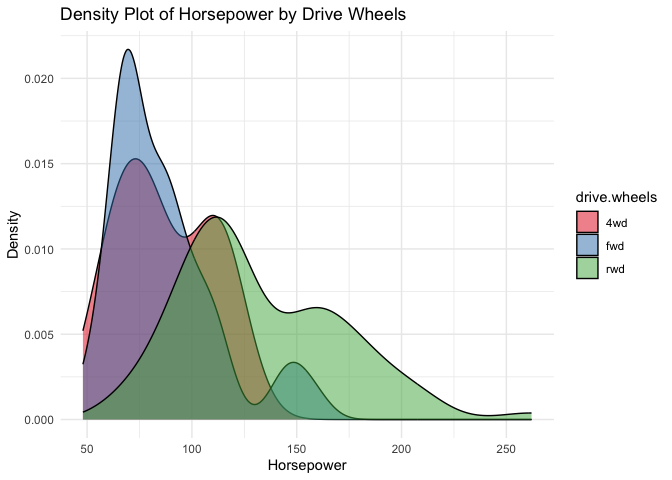
\includegraphics{AnabolicStatistics_files/figure-latex/unnamed-chunk-7-1.pdf}

\begin{Shaded}
\begin{Highlighting}[]
\CommentTok{\# Scatter plot}
\FunctionTok{ggplot}\NormalTok{(cardata, }\FunctionTok{aes}\NormalTok{(}\AttributeTok{x =}\NormalTok{ engine.size, }\AttributeTok{y =}\NormalTok{ horsepower)) }\SpecialCharTok{+}
  \FunctionTok{geom\_point}\NormalTok{() }\SpecialCharTok{+}
  \FunctionTok{labs}\NormalTok{(}\AttributeTok{title =} \StringTok{"Scatter Plot of Engine Size vs Horsepower"}\NormalTok{,}
       \AttributeTok{x =} \StringTok{"Engine Size"}\NormalTok{,}
       \AttributeTok{y =} \StringTok{"Horsepower"}\NormalTok{) }\SpecialCharTok{+}
  \FunctionTok{theme\_minimal}\NormalTok{()}
\end{Highlighting}
\end{Shaded}

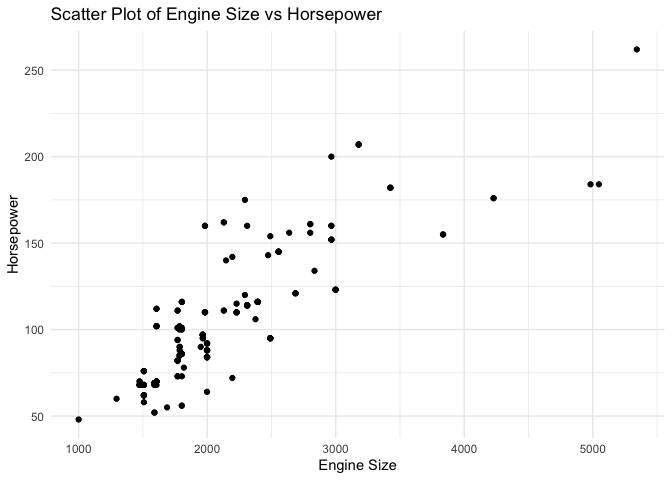
\includegraphics{AnabolicStatistics_files/figure-latex/unnamed-chunk-7-2.pdf}

\subsection{Zaključak}\label{zakljuux10dak}

Na temelju provedenih analiza, zaključujemo da tip pogona automobila
značajno utječe na snagu motora. Rezultati Kruskal-Wallis testa i
t-testova pokazali su da postoje statistički značajne razlike u snazi
motora između vozila s različitim vrstama pogona. Vozila sa zadnjim
pogonom (RWD) obično imaju veću snagu motora u usporedbi s vozilima s
prednjim pogonom (FWD) i pogonom na sva četiri kotača (4WD). Ovo je
vidljivo iz visokih vrijednosti medijana i veće varijance u snazi motora
kod RWD vozila, što ukazuje na sklonost prema performansama i sportskoj
orijentaciji.

S druge strane, vozila s prednjim pogonom (FWD) i pogonom na sva četiri
kotača (4WD) pokazala su sličnu prosječnu snagu motora, što ukazuje na
to da su ta vozila više usmjerena na uravnoteženost između ekonomičnosti
i sposobnosti terenske vožnje. Ovo je potvrđeno t-testom između FWD i
4WD kategorija, gdje nije bilo statistički značajne razlike u prosječnoj
snazi motora. Vizualne analize, uključujući histograme, boxplotove i
density plot, dodatno su potvrdile ove nalaze.

U odgovoru na postavljeno pitanje, možemo zaključiti da automobili s
prednjim pogonom (FWD) generalno nemaju veću snagu motora u usporedbi s
ostalim vrstama pogona. U stvarnosti, automobili s RWD pogonom imaju
tendenciju posjedovanja veće snage motora, dok su FWD i 4WD automobili
sličniji po prosječnoj snazi motora.

\section{Pitanje 2 - Razlike u potrošnji automobila prema
regiji}\label{pitanje-2---razlike-u-potroux161nji-automobila-prema-regiji}

\textbf{Postoje li razlike u potrošnji automobila prema regiji kojoj
pripada proizvođač?}

\subsection{Uvod}\label{uvod-1}

Da odgovorimo na ovo pitanje, moramo analizirati podatke potrošnje
goriva na 3 kontinenta. Zbog činjenice da imamo više od 2 regije,
analiza varijance (ANOVA) će biti naš odabir modeliranja umjesto
t-testa, ali prije toga ćemo morati testirati uvjete ANOVA-e.

Učitavanje podataka:

\begin{Shaded}
\begin{Highlighting}[]
\NormalTok{path }\OtherTok{\textless{}{-}} \StringTok{"car\_specifications.csv"}
\NormalTok{data }\OtherTok{\textless{}{-}} \FunctionTok{read.csv}\NormalTok{(path)}

\NormalTok{data}\SpecialCharTok{$}\NormalTok{continent }\OtherTok{=} \FunctionTok{as.factor}\NormalTok{(data}\SpecialCharTok{$}\NormalTok{continent)}
\NormalTok{data}\SpecialCharTok{$}\NormalTok{country }\OtherTok{=} \FunctionTok{as.factor}\NormalTok{(data}\SpecialCharTok{$}\NormalTok{country)}
\FunctionTok{head}\NormalTok{(data)}
\end{Highlighting}
\end{Shaded}

\begin{verbatim}
##         make aspiration num.of.doors  body.style drive.wheels engine.location
## 1 Alfa Romeo        std          two convertible          rwd           front
## 2 Alfa Romeo        std          two convertible          rwd           front
## 3 Alfa Romeo        std          two   hatchback          rwd           front
## 4       Audi        std         four       sedan          fwd           front
## 5       Audi        std         four       sedan          4wd           front
## 6       Audi        std          two       sedan          fwd           front
##   wheel.base length width height curb.weight engine.type num.of.cylinders
## 1      225.0  428.8 162.8  124.0        1156        dohc             four
## 2      225.0  428.8 162.8  124.0        1156        dohc             four
## 3      240.0  434.8 166.4  133.1        1280        ohcv              six
## 4      253.5  448.6 168.1  137.9        1060         ohc             four
## 5      252.5  448.6 168.7  137.9        1281         ohc             five
## 6      253.5  450.3 168.4  134.9        1137         ohc             five
##   engine.size fuel.system bore stroke compression.ratio horsepower peak.rpm
## 1        2130        mpfi 8.81   6.81               9.0        111     5000
## 2        2130        mpfi 8.81   6.81               9.0        111     5000
## 3        2491        mpfi 6.81   8.81               9.0        154     5000
## 4        1786        mpfi 8.10   8.64              10.0        102     5500
## 5        2229        mpfi 8.10   8.64               8.0        115     5500
## 6        2229        mpfi 8.10   8.64               8.5        110     5500
##   price city.L.100km highway.L.100km   fuel country continent
## 1 13495        11.19            8.70 petrol   Italy    Europe
## 2 16500        11.19            8.70 petrol   Italy    Europe
## 3 16500        12.37            9.04 petrol   Italy    Europe
## 4 13950         9.79            7.83 petrol Germany    Europe
## 5 17450        13.06           10.68 petrol Germany    Europe
## 6 15250        12.37            9.40 petrol Germany    Europe
\end{verbatim}

Nama su relevantni stupci `city.L.100km', `highway.L.100km' i
`continent'

\subsection{Usporedba sredina}\label{usporedba-sredina}

\textbf{\emph{Provjera aritmetičkih sredina}} Prije nego krenemo sa
ANOVA-om, možemo prvo usporediti aritmetičke sredine podataka. Ovo nije
dovoljno da radimo bilo kakve konkretne zaključke, ali nam daje uvid u
što bi možda očekivali. Također ćemo izračunati varijancu i standardnu
devijaciju da imamo bolju ideju o izgledu raspršenosti podataka.
Provjerimo sredine za pojedine kontinente sa boxplotom i sveukupnu
sredinu i varijance kroz ispis:

\begin{Shaded}
\begin{Highlighting}[]
\NormalTok{continents }\OtherTok{=} \FunctionTok{unique}\NormalTok{(data}\SpecialCharTok{$}\NormalTok{continent) }\CommentTok{\#lista svih kontinenta}

\NormalTok{overallMeanCity }\OtherTok{=} \FunctionTok{mean}\NormalTok{(data}\SpecialCharTok{$}\NormalTok{city.L}\FloatTok{.100}\NormalTok{km)}
\NormalTok{overallMeanHighway }\OtherTok{=} \FunctionTok{mean}\NormalTok{(data}\SpecialCharTok{$}\NormalTok{highway.L}\FloatTok{.100}\NormalTok{km)}
\NormalTok{overallVarCity }\OtherTok{=} \FunctionTok{var}\NormalTok{(data}\SpecialCharTok{$}\NormalTok{city.L}\FloatTok{.100}\NormalTok{km)}
\NormalTok{overallVarHighway }\OtherTok{=} \FunctionTok{var}\NormalTok{(data}\SpecialCharTok{$}\NormalTok{highway.L}\FloatTok{.100}\NormalTok{km)}

\FunctionTok{cat}\NormalTok{(}\StringTok{"}\SpecialCharTok{\textbackslash{}n}\StringTok{"}\NormalTok{)}
\FunctionTok{print}\NormalTok{(}\FunctionTok{sprintf}\NormalTok{(}\StringTok{"Aritmetička sredina potrošnje goriva u gradu: \%f"}\NormalTok{,overallMeanCity))}
\FunctionTok{print}\NormalTok{(}\FunctionTok{sprintf}\NormalTok{(}\StringTok{"Aritmetička sredina potrošnje goriva na autocestama: \%f"}\NormalTok{,overallMeanHighway))}

\FunctionTok{print}\NormalTok{(}\FunctionTok{sprintf}\NormalTok{(}\StringTok{"Sveukupna varijanca za gradove: \%f"}\NormalTok{,overallVarCity))}
\FunctionTok{print}\NormalTok{(}\FunctionTok{sprintf}\NormalTok{(}\StringTok{"Standardna devijacija: \%f"}\NormalTok{,}\FunctionTok{sqrt}\NormalTok{(overallVarCity)))}

\FunctionTok{print}\NormalTok{(}\FunctionTok{sprintf}\NormalTok{(}\StringTok{"Sveukupna varijanca za autoceste: \%f"}\NormalTok{,overallVarHighway))}
\FunctionTok{print}\NormalTok{(}\FunctionTok{sprintf}\NormalTok{(}\StringTok{"Standardna devijacija: \%f"}\NormalTok{,}\FunctionTok{sqrt}\NormalTok{(overallVarHighway)))}

\FunctionTok{boxplot}\NormalTok{(data}\SpecialCharTok{$}\NormalTok{city.L}\FloatTok{.100}\NormalTok{km }\SpecialCharTok{\textasciitilde{}}\NormalTok{ data}\SpecialCharTok{$}\NormalTok{continent)}
\end{Highlighting}
\end{Shaded}

\includegraphics{AnabolicStatistics_files/figure-latex/unnamed-chunk-9-1.pdf}

\begin{Shaded}
\begin{Highlighting}[]
\FunctionTok{boxplot}\NormalTok{(data}\SpecialCharTok{$}\NormalTok{highway.L}\FloatTok{.100}\NormalTok{km }\SpecialCharTok{\textasciitilde{}}\NormalTok{ data}\SpecialCharTok{$}\NormalTok{continent)}
\end{Highlighting}
\end{Shaded}

\includegraphics{AnabolicStatistics_files/figure-latex/unnamed-chunk-9-2.pdf}

\begin{verbatim}
## 
## [1] "Aritmetička sredina potrošnje goriva u gradu: 9.943582"
## [1] "Aritmetička sredina potrošnje goriva na autocestama: 8.043433"
## [1] "Sveukupna varijanca za gradove: 6.429238"
## [1] "Standardna devijacija: 2.535594"
## [1] "Sveukupna varijanca za autoceste: 3.390360"
## [1] "Standardna devijacija: 1.841293"
\end{verbatim}

Već vidimo da je potrošnja u Europi u prosjeku veća nego druga dva
kontinenta. Osim toga vidimo da je i disperzija nešto veća.

\#Uvjeti za ANOVA-u Podsjetimo se. Želimo testirati ima li značajno
odstupanje u sredinama potrošnje goriva na 3 kontinenta i zato prirodno
biramo ANOVA-u. Kako bi proveli ANOVA test na podacima, prvo moramo biti
sigurni da dani podaci zadovoljavaju sljedeće uvjete: 1. Normalnost 2.
Nezavisnost 3. Homogenost varijanci

\section{Testiranje normalnosti}\label{testiranje-normalnosti}

Prvo ćemo proveti test normalnosti. Zanimaju nas tablice za potrošnju
goriva u gradu i na autocesti za svaki kontinent. Koristit ćemo
Lilliefors test koji se temelji na Kolmogorov-Smirnov testu i Q-Q plot
za vizualizaciju. Postavljamo hipoteze: \[\begin{aligned}
H_0 &: Dani\ podaci\ za\ potrošnju\ goriva\ imaju\ normalnu\ distribuciju\\
H_1 &: \neg H0
\end{aligned}\]

Provedimo test:

\begin{Shaded}
\begin{Highlighting}[]
\FunctionTok{require}\NormalTok{(nortest) }\CommentTok{\#potrebna biblioteka}

\ControlFlowTok{for}\NormalTok{ (continent }\ControlFlowTok{in}\NormalTok{ continents) \{}
  \FunctionTok{print}\NormalTok{(}\FunctionTok{paste}\NormalTok{(}\StringTok{"For continent:"}\NormalTok{,continent))}
  \FunctionTok{print}\NormalTok{(}\FunctionTok{lillie.test}\NormalTok{(data}\SpecialCharTok{$}\NormalTok{city.L}\FloatTok{.100}\NormalTok{km[data}\SpecialCharTok{$}\NormalTok{continent }\SpecialCharTok{==}\NormalTok{ continent]))}
  \FunctionTok{print}\NormalTok{(}\FunctionTok{lillie.test}\NormalTok{(data}\SpecialCharTok{$}\NormalTok{highway.L}\FloatTok{.100}\NormalTok{km[data}\SpecialCharTok{$}\NormalTok{continent }\SpecialCharTok{==}\NormalTok{ continent]))}
\NormalTok{  titleHighway }\OtherTok{=} \FunctionTok{paste}\NormalTok{(continent,}\StringTok{", highway"}\NormalTok{)}
\NormalTok{  titleCity }\OtherTok{=} \FunctionTok{paste}\NormalTok{(continent,}\StringTok{", city"}\NormalTok{)}
  \FunctionTok{hist}\NormalTok{(data}\SpecialCharTok{$}\NormalTok{highway.L}\FloatTok{.100}\NormalTok{km[data}\SpecialCharTok{$}\NormalTok{continent }\SpecialCharTok{==}\NormalTok{ continent],}\AttributeTok{main=}\NormalTok{titleHighway)}
  \FunctionTok{hist}\NormalTok{(data}\SpecialCharTok{$}\NormalTok{city.L}\FloatTok{.100}\NormalTok{km[data}\SpecialCharTok{$}\NormalTok{continent }\SpecialCharTok{==}\NormalTok{ continent],}\AttributeTok{main=}\NormalTok{titleCity)}
\NormalTok{\}}
\end{Highlighting}
\end{Shaded}

\includegraphics{AnabolicStatistics_files/figure-latex/unnamed-chunk-10-1.pdf}
\includegraphics{AnabolicStatistics_files/figure-latex/unnamed-chunk-10-2.pdf}
\includegraphics{AnabolicStatistics_files/figure-latex/unnamed-chunk-10-3.pdf}
\includegraphics{AnabolicStatistics_files/figure-latex/unnamed-chunk-10-4.pdf}
\includegraphics{AnabolicStatistics_files/figure-latex/unnamed-chunk-10-5.pdf}
\includegraphics{AnabolicStatistics_files/figure-latex/unnamed-chunk-10-6.pdf}

\begin{verbatim}
## [1] "For continent: Europe"
## 
##  Lilliefors (Kolmogorov-Smirnov) normality test
## 
## data:  data$city.L.100km[data$continent == continent]
## D = 0.11082, p-value = 0.02499
## 
## 
##  Lilliefors (Kolmogorov-Smirnov) normality test
## 
## data:  data$highway.L.100km[data$continent == continent]
## D = 0.17288, p-value = 9.739e-06
## 
## [1] "For continent: North America"
## 
##  Lilliefors (Kolmogorov-Smirnov) normality test
## 
## data:  data$city.L.100km[data$continent == continent]
## D = 0.2557, p-value = 0.001348
## 
## 
##  Lilliefors (Kolmogorov-Smirnov) normality test
## 
## data:  data$highway.L.100km[data$continent == continent]
## D = 0.28537, p-value = 0.0001587
## 
## [1] "For continent: Asia"
## 
##  Lilliefors (Kolmogorov-Smirnov) normality test
## 
## data:  data$city.L.100km[data$continent == continent]
## D = 0.15718, p-value = 7.516e-07
## 
## 
##  Lilliefors (Kolmogorov-Smirnov) normality test
## 
## data:  data$highway.L.100km[data$continent == continent]
## D = 0.14449, p-value = 9.635e-06
\end{verbatim}

Dobili smo vrlo male p-vrijednosti. Sve su signifikantne na barem 0.05
razini, a većina je i ekstremnije od toga. Ovime možemo uvjereno
odbaciti H0 i zaključiti kako podaci nisu normalno distribuirani. Osim
toga, histogrami očito pokazuju kako podaci ne prate Gaussovu krivulju.
Manjak normalnosti možemo vidjeti i na Q-Q plotu:

\begin{Shaded}
\begin{Highlighting}[]
\FunctionTok{qqnorm}\NormalTok{(data}\SpecialCharTok{$}\NormalTok{highway.L}\FloatTok{.100}\NormalTok{km[data}\SpecialCharTok{$}\NormalTok{continent }\SpecialCharTok{==} \StringTok{"Asia"}\NormalTok{],}\AttributeTok{main=}\StringTok{"Asia, highways"}\NormalTok{)}
\FunctionTok{qqline}\NormalTok{(data}\SpecialCharTok{$}\NormalTok{highway.L}\FloatTok{.100}\NormalTok{km[data}\SpecialCharTok{$}\NormalTok{continent }\SpecialCharTok{==} \StringTok{"Asia"}\NormalTok{])}
\end{Highlighting}
\end{Shaded}

\includegraphics{AnabolicStatistics_files/figure-latex/unnamed-chunk-11-1.pdf}

\begin{Shaded}
\begin{Highlighting}[]
\FunctionTok{qqnorm}\NormalTok{(data}\SpecialCharTok{$}\NormalTok{city.L}\FloatTok{.100}\NormalTok{km[data}\SpecialCharTok{$}\NormalTok{continent }\SpecialCharTok{==} \StringTok{"Asia"}\NormalTok{],}\AttributeTok{main =} \StringTok{"Asia, cities"}\NormalTok{)}
\FunctionTok{qqline}\NormalTok{(data}\SpecialCharTok{$}\NormalTok{city.L}\FloatTok{.100}\NormalTok{km[data}\SpecialCharTok{$}\NormalTok{continent }\SpecialCharTok{==} \StringTok{"Asia"}\NormalTok{])}
\end{Highlighting}
\end{Shaded}

\includegraphics{AnabolicStatistics_files/figure-latex/unnamed-chunk-11-2.pdf}

\begin{Shaded}
\begin{Highlighting}[]
\FunctionTok{qqnorm}\NormalTok{(data}\SpecialCharTok{$}\NormalTok{highway.L}\FloatTok{.100}\NormalTok{km[data}\SpecialCharTok{$}\NormalTok{continent }\SpecialCharTok{==} \StringTok{"North America"}\NormalTok{],}\AttributeTok{main =} \StringTok{"NA,highways"}\NormalTok{)}
\FunctionTok{qqline}\NormalTok{(data}\SpecialCharTok{$}\NormalTok{highway.L}\FloatTok{.100}\NormalTok{km[data}\SpecialCharTok{$}\NormalTok{continent }\SpecialCharTok{==} \StringTok{"North America"}\NormalTok{])}
\end{Highlighting}
\end{Shaded}

\includegraphics{AnabolicStatistics_files/figure-latex/unnamed-chunk-11-3.pdf}

\begin{Shaded}
\begin{Highlighting}[]
\FunctionTok{qqnorm}\NormalTok{(data}\SpecialCharTok{$}\NormalTok{city.L}\FloatTok{.100}\NormalTok{km[data}\SpecialCharTok{$}\NormalTok{continent }\SpecialCharTok{==} \StringTok{"North America"}\NormalTok{],}\AttributeTok{main =} \StringTok{"NA, cities"}\NormalTok{)}
\FunctionTok{qqline}\NormalTok{(data}\SpecialCharTok{$}\NormalTok{city.L}\FloatTok{.100}\NormalTok{km[data}\SpecialCharTok{$}\NormalTok{continent }\SpecialCharTok{==} \StringTok{"North America"}\NormalTok{])}
\end{Highlighting}
\end{Shaded}

\includegraphics{AnabolicStatistics_files/figure-latex/unnamed-chunk-11-4.pdf}

\begin{Shaded}
\begin{Highlighting}[]
\FunctionTok{qqnorm}\NormalTok{(data}\SpecialCharTok{$}\NormalTok{highway.L}\FloatTok{.100}\NormalTok{km[data}\SpecialCharTok{$}\NormalTok{continent }\SpecialCharTok{==} \StringTok{"Europe"}\NormalTok{],}\AttributeTok{main =} \StringTok{"Europe, highways"}\NormalTok{)}
\FunctionTok{qqline}\NormalTok{(data}\SpecialCharTok{$}\NormalTok{highway.L}\FloatTok{.100}\NormalTok{km[data}\SpecialCharTok{$}\NormalTok{continent }\SpecialCharTok{==} \StringTok{"Europe"}\NormalTok{])}
\end{Highlighting}
\end{Shaded}

\includegraphics{AnabolicStatistics_files/figure-latex/unnamed-chunk-11-5.pdf}

\begin{Shaded}
\begin{Highlighting}[]
\FunctionTok{qqnorm}\NormalTok{(data}\SpecialCharTok{$}\NormalTok{city.L}\FloatTok{.100}\NormalTok{km[data}\SpecialCharTok{$}\NormalTok{continent }\SpecialCharTok{==} \StringTok{"Europe"}\NormalTok{],}\AttributeTok{main =} \StringTok{"Europe, cities"}\NormalTok{)}
\FunctionTok{qqline}\NormalTok{(data}\SpecialCharTok{$}\NormalTok{city.L}\FloatTok{.100}\NormalTok{km[data}\SpecialCharTok{$}\NormalTok{continent }\SpecialCharTok{==} \StringTok{"Europe"}\NormalTok{])}
\end{Highlighting}
\end{Shaded}

\includegraphics{AnabolicStatistics_files/figure-latex/unnamed-chunk-11-6.pdf}

Iako KS test i Q-Q plotovi nedaju dobre izglede za normalnost, vidimo na
plotovima da podaci u sredini približno prate fitted liniju. Za sada
ćemo reći da je ovo `dovoljno dobro' i nastaviti sa Bartlettovim testom,
ali ćemo kasnije napraviti i Kruskal-Wallis test kako bi bili sigurni.

\[ \begin{aligned}
  H_0 & : \sigma_1^2 = \sigma_2^2= \sigma_3^2 \\
  H_1 & : \text{barem dvije varijance nisu iste}.
\end{aligned} \]

\begin{Shaded}
\begin{Highlighting}[]
\NormalTok{bartlettCity}\OtherTok{=}\FunctionTok{bartlett.test}\NormalTok{(data}\SpecialCharTok{$}\NormalTok{city.L}\FloatTok{.100}\NormalTok{km }\SpecialCharTok{\textasciitilde{}}\NormalTok{ data}\SpecialCharTok{$}\NormalTok{continent)}
\NormalTok{bartlettHighway }\OtherTok{=} \FunctionTok{bartlett.test}\NormalTok{(data}\SpecialCharTok{$}\NormalTok{highway.L}\FloatTok{.100}\NormalTok{km }\SpecialCharTok{\textasciitilde{}}\NormalTok{ data}\SpecialCharTok{$}\NormalTok{continent)}
\FunctionTok{print}\NormalTok{(bartlettCity)}
\FunctionTok{print}\NormalTok{(bartlettHighway)}

\ControlFlowTok{for}\NormalTok{(continent }\ControlFlowTok{in}\NormalTok{ continents) \{}
  \FunctionTok{print}\NormalTok{(}\FunctionTok{var}\NormalTok{(data}\SpecialCharTok{$}\NormalTok{highway.L}\FloatTok{.100}\NormalTok{km[data}\SpecialCharTok{$}\NormalTok{continent }\SpecialCharTok{==}\NormalTok{ continent]))}
  \FunctionTok{print}\NormalTok{(}\FunctionTok{var}\NormalTok{(data}\SpecialCharTok{$}\NormalTok{city.L}\FloatTok{.100}\NormalTok{km[data}\SpecialCharTok{$}\NormalTok{continent }\SpecialCharTok{==}\NormalTok{ continent]))}
\NormalTok{\}}
\end{Highlighting}
\end{Shaded}

\begin{verbatim}
## 
##  Bartlett test of homogeneity of variances
## 
## data:  data$city.L.100km by data$continent
## Bartlett's K-squared = 3.278, df = 2, p-value = 0.1942
## 
## 
##  Bartlett test of homogeneity of variances
## 
## data:  data$highway.L.100km by data$continent
## Bartlett's K-squared = 9.1482, df = 2, p-value = 0.01032
## 
## [1] 3.700244
## [1] 6.154051
## [1] 2.416816
## [1] 4.810641
## [1] 1.942657
## [1] 4.176483
\end{verbatim}

Jedan test ima veliku p-vrijednost, drugi malu. Opet, ovo ne izgleda
obečavajuće za ANOVA test ali za sad ćemo reći da je `dovoljno dobro'.
ANOVA hipoteze: \[\begin{aligned}
H_0 &:\ Očekivana\ vrijednost\ potrošnje\ goriva\ po\ kontinentima\ je\ jednaka\\
H_1 &: Barem\ jedna\ očekivana\ vrijednost\ se\ razlikuje\ od\ ostalih
\end{aligned}\]

\begin{Shaded}
\begin{Highlighting}[]
\NormalTok{aC }\OtherTok{=} \FunctionTok{aov}\NormalTok{(data}\SpecialCharTok{$}\NormalTok{city.L}\FloatTok{.100}\NormalTok{km }\SpecialCharTok{\textasciitilde{}}\NormalTok{ data}\SpecialCharTok{$}\NormalTok{continent)}
\NormalTok{aH }\OtherTok{=} \FunctionTok{aov}\NormalTok{(data}\SpecialCharTok{$}\NormalTok{highway.L}\FloatTok{.100}\NormalTok{km }\SpecialCharTok{\textasciitilde{}}\NormalTok{ data}\SpecialCharTok{$}\NormalTok{continent)}

\FunctionTok{summary}\NormalTok{(aC)}
\FunctionTok{print}\NormalTok{(}\StringTok{"============================================================"}\NormalTok{)}
\FunctionTok{summary}\NormalTok{(aH)}
\end{Highlighting}
\end{Shaded}

\begin{verbatim}
##                 Df Sum Sq Mean Sq F value   Pr(>F)    
## data$continent   2  302.5  151.25   30.45 2.94e-12 ***
## Residuals      198  983.4    4.97                     
## ---
## Signif. codes:  0 '***' 0.001 '**' 0.01 '*' 0.05 '.' 0.1 ' ' 1
## [1] "============================================================"
##                 Df Sum Sq Mean Sq F value   Pr(>F)    
## data$continent   2  156.1   78.06   29.61 5.62e-12 ***
## Residuals      198  522.0    2.64                     
## ---
## Signif. codes:  0 '***' 0.001 '**' 0.01 '*' 0.05 '.' 0.1 ' ' 1
\end{verbatim}

Dobili smo male p-vrijednosti za oba testa. Ovo sugerira da postoje
razlike u srednjim vrijednostima. Probajmo prilagoditi model:

\begin{Shaded}
\begin{Highlighting}[]
\NormalTok{modelC }\OtherTok{=} \FunctionTok{lm}\NormalTok{(data}\SpecialCharTok{$}\NormalTok{city.L}\FloatTok{.100}\NormalTok{km }\SpecialCharTok{\textasciitilde{}}\NormalTok{ data}\SpecialCharTok{$}\NormalTok{continent)}
\FunctionTok{summary}\NormalTok{(modelC)}
\FunctionTok{print}\NormalTok{(}\StringTok{"============================================================"}\NormalTok{)}
\NormalTok{modelH }\OtherTok{=} \FunctionTok{lm}\NormalTok{(data}\SpecialCharTok{$}\NormalTok{highway.L}\FloatTok{.100}\NormalTok{km }\SpecialCharTok{\textasciitilde{}}\NormalTok{ data}\SpecialCharTok{$}\NormalTok{continent)}
\FunctionTok{summary}\NormalTok{(modelH)}
\end{Highlighting}
\end{Shaded}

\begin{verbatim}
## 
## Call:
## lm(formula = data$city.L.100km ~ data$continent)
## 
## Residuals:
##     Min      1Q  Median      3Q     Max 
## -5.1808 -1.5434 -0.3408  0.8392  6.5492 
## 
## Coefficients:
##                             Estimate Std. Error t value Pr(>|t|)    
## (Intercept)                   9.1234     0.2154  42.347  < 2e-16 ***
## data$continentEurope          2.4074     0.3369   7.145 1.68e-11 ***
## data$continentNorth America  -0.6644     0.5429  -1.224    0.223    
## ---
## Signif. codes:  0 '***' 0.001 '**' 0.01 '*' 0.05 '.' 0.1 ' ' 1
## 
## Residual standard error: 2.229 on 198 degrees of freedom
## Multiple R-squared:  0.2352, Adjusted R-squared:  0.2275 
## F-statistic: 30.45 on 2 and 198 DF,  p-value: 2.941e-12
## 
## [1] "============================================================"
## 
## Call:
## lm(formula = data$highway.L.100km ~ data$continent)
## 
## Residuals:
##     Min      1Q  Median      3Q     Max 
## -4.0700 -1.1154 -0.1254  0.6100  5.5100 
## 
## Coefficients:
##                             Estimate Std. Error t value Pr(>|t|)    
## (Intercept)                   7.4654     0.1570  47.562  < 2e-16 ***
## data$continentEurope          1.7146     0.2455   6.985 4.24e-11 ***
## data$continentNorth America  -0.5349     0.3955  -1.352    0.178    
## ---
## Signif. codes:  0 '***' 0.001 '**' 0.01 '*' 0.05 '.' 0.1 ' ' 1
## 
## Residual standard error: 1.624 on 198 degrees of freedom
## Multiple R-squared:  0.2302, Adjusted R-squared:  0.2225 
## F-statistic: 29.61 on 2 and 198 DF,  p-value: 5.619e-12
\end{verbatim}

Vidimo da smo dobili malu p-vrijednost, ali i mali R\^{}2. Ovo sugerira
da iako model ne objašnjava najbolje dane podatke, barem jedna nezavisna
varijabla je statistički vezana vezana sa zavisnim.

\#Kruskal-Wallis test Okrećemo se alternativi ANOVA testa,
Kruskal-Wallis test. To je neparametarski test pa ne trebamo da nam
podaci prate određenu distribuciju. Jedini uvjet je da je broj podataka
barem 5. Hipoteze se postavljaju na isti način kao u ANOVA-i.

Hipoteze: \[\begin{aligned}
H_0 &:\ Očekivana\ vrijednost\ potrošnje\ goriva\ po\ kontinentima\ je\ jednaka\\
H_1 &: Barem\ jedna\ očekivana\ vrijednost\ se\ razlikuje\ od\ ostalih
\end{aligned}\] Ovu istu hipotezu p Ovu istu hipotezu postavljamo za
gradove i autoceste te zbog toga provodimo test dvaput.

Provedimo Kruskal-Wallis test:

\begin{Shaded}
\begin{Highlighting}[]
\NormalTok{filteredDataHighway }\OtherTok{=} \FunctionTok{list}\NormalTok{(}\AttributeTok{Asia\_Highway =}\NormalTok{ data}\SpecialCharTok{$}\NormalTok{highway.L}\FloatTok{.100}\NormalTok{km[data}\SpecialCharTok{$}\NormalTok{continent }\SpecialCharTok{==} \StringTok{"Asia"}\NormalTok{], }\AttributeTok{NA\_Highway =}\NormalTok{ data}\SpecialCharTok{$}\NormalTok{highway.L}\FloatTok{.100}\NormalTok{km[data}\SpecialCharTok{$}\NormalTok{continent }\SpecialCharTok{==} \StringTok{"North America"}\NormalTok{], }\AttributeTok{Europe\_Highway =}\NormalTok{ data}\SpecialCharTok{$}\NormalTok{highway.L}\FloatTok{.100}\NormalTok{km[data}\SpecialCharTok{$}\NormalTok{continent }\SpecialCharTok{==} \StringTok{"Europe"}\NormalTok{])}
\NormalTok{filteredDataCity }\OtherTok{=} \FunctionTok{list}\NormalTok{(}\AttributeTok{Asia\_City =}\NormalTok{ data}\SpecialCharTok{$}\NormalTok{city.L}\FloatTok{.100}\NormalTok{km[data}\SpecialCharTok{$}\NormalTok{continent }\SpecialCharTok{==} \StringTok{"Asia"}\NormalTok{], }\AttributeTok{NA\_City =}\NormalTok{ data}\SpecialCharTok{$}\NormalTok{city.L}\FloatTok{.100}\NormalTok{km[data}\SpecialCharTok{$}\NormalTok{continent }\SpecialCharTok{==} \StringTok{"North America"}\NormalTok{], }\AttributeTok{Europe\_City =}\NormalTok{ data}\SpecialCharTok{$}\NormalTok{city.L}\FloatTok{.100}\NormalTok{km[data}\SpecialCharTok{$}\NormalTok{continent }\SpecialCharTok{==} \StringTok{"Europe"}\NormalTok{])}

\NormalTok{kruskalHighway }\OtherTok{=} \FunctionTok{kruskal.test}\NormalTok{(filteredDataHighway)}
\NormalTok{kruskalCity }\OtherTok{=} \FunctionTok{kruskal.test}\NormalTok{(filteredDataCity)}
\FunctionTok{print}\NormalTok{(kruskalHighway)}
\end{Highlighting}
\end{Shaded}

\begin{verbatim}
## 
##  Kruskal-Wallis rank sum test
## 
## data:  filteredDataHighway
## Kruskal-Wallis chi-squared = 46.203, df = 2, p-value = 9.272e-11
\end{verbatim}

Provjerimo prvo rezultat za potrošnju na autocestama. Dobili smo vrlo
malu p-vrijednost, praktički je jednaka nuli, dakle bez sumnje
odbacujemo H0 i zaključujemo da se barem jedna očekivana vrijednost
razlikuje od ostalih.

Provjerimo sad rezultat za gradove:

\begin{Shaded}
\begin{Highlighting}[]
\FunctionTok{print}\NormalTok{(kruskalCity)}
\end{Highlighting}
\end{Shaded}

\begin{verbatim}
## 
##  Kruskal-Wallis rank sum test
## 
## data:  filteredDataCity
## Kruskal-Wallis chi-squared = 49.079, df = 2, p-value = 2.201e-11
\end{verbatim}

Opet imamo p-vrijednost koja je efektivno jednaka nuli. Za potrošnju u
gradovima također odbacujemo H0.

Na temelju boxplotova koje smo ranije vidjeli, najvjerojatnije su podaci
za Europu zaslužni za odbijanje H0. Možemo koristiti Dunnov test da
vidimo između kojih grupa su razlike značajne. Dunnov test ima istu
hipotezu kao Kruskal-Wallis test.

\begin{Shaded}
\begin{Highlighting}[]
\FunctionTok{require}\NormalTok{(dunn.test)}
\end{Highlighting}
\end{Shaded}

\begin{verbatim}
## Loading required package: dunn.test
\end{verbatim}

\begin{Shaded}
\begin{Highlighting}[]
\NormalTok{dunn }\OtherTok{=} \FunctionTok{dunn.test}\NormalTok{(data}\SpecialCharTok{$}\NormalTok{highway.L}\FloatTok{.100}\NormalTok{km , }\AttributeTok{g =}\NormalTok{ data}\SpecialCharTok{$}\NormalTok{continent,}\AttributeTok{method=}\StringTok{"bonferroni"}\NormalTok{)}
\FunctionTok{print}\NormalTok{(dunn)}
\NormalTok{dunn }\OtherTok{=} \FunctionTok{dunn.test}\NormalTok{(data}\SpecialCharTok{$}\NormalTok{city.L}\FloatTok{.100}\NormalTok{km, }\AttributeTok{g =}\NormalTok{ data}\SpecialCharTok{$}\NormalTok{continent, }\AttributeTok{method =} \StringTok{"bonferroni"}\NormalTok{)}
\end{Highlighting}
\end{Shaded}

\begin{verbatim}
##   Kruskal-Wallis rank sum test
## 
## data: x and group
## Kruskal-Wallis chi-squared = 46.2028, df = 2, p-value = 0
## 
## 
##                            Comparison of x by group                            
##                                  (Bonferroni)                                  
## Col Mean-|
## Row Mean |       Asia     Europe
## ---------+----------------------
##   Europe |  -6.059794
##          |    0.0000*
##          |
## North Am |   1.440839   5.028198
##          |     0.2244    0.0000*
## 
## alpha = 0.05
## Reject Ho if p <= alpha/2
## $chi2
## [1] 46.20277
## 
## $Z
## [1] -6.059794  1.440840  5.028199
## 
## $P
## [1] 6.814784e-10 7.481500e-02 2.475542e-07
## 
## $P.adjusted
## [1] 2.044435e-09 2.244450e-01 7.426625e-07
## 
## $comparisons
## [1] "Asia - Europe"          "Asia - North America"   "Europe - North America"
## 
##   Kruskal-Wallis rank sum test
## 
## data: x and group
## Kruskal-Wallis chi-squared = 49.0792, df = 2, p-value = 0
## 
## 
##                            Comparison of x by group                            
##                                  (Bonferroni)                                  
## Col Mean-|
## Row Mean |       Asia     Europe
## ---------+----------------------
##   Europe |  -6.382981
##          |    0.0000*
##          |
## North Am |   1.173223   4.963401
##          |     0.3611    0.0000*
## 
## alpha = 0.05
## Reject Ho if p <= alpha/2
\end{verbatim}

Zanima nas ``p-adjusted'' redak koji se također može vidjeti u
tablici(drugi redak u svakoj čeliji). Za oba testa imamo isti zaključak
Vidimo da je p-adjusted za North\_America-Asia relativno velik i nije
signifikantan na niti jednoj tipičnoj razini. Međutim, imamo vrlo male
p-adjusted vrijednosti između Europe i bilo kojeg drugog kontinenta.
Ovime možemo zaključiti da je odbijanje nul hipoteze Kruskal-Wallis
testa bilo primarno zbog razine potrošnje u Europi.

\subsection{Subregionalno}\label{subregionalno}

\textbf{Testiranje među regijama u Europi} Budući da Azija i Sjeverna
Amerika imaju relativno slične potrošnje, ne zanima nas detaljnije
subregionalno testiranje. Osim toga, ti kontinenti imaju samo po jednu
državu u podacima, dakle ni ne možemo podjeliti na manje regije.
Međutim, Europu, koja je imala poprilično veliku potrošnju goriva i
mnogo država, možemo podijeliti na manje regije, no ne možemo testirati
na pojedinim državama jer za neke nemamo dovoljno podataka. Opet ćemo
napraviti Kruskal-Wallis test i, po potrebi, Dunnov test. Ovime možemo
probati zaključiti ako se u nekim regijama više troši.

\textbf{\emph{Podjela na subregije}} Trebamo odrediti kako želimo
grupirati države. Ciljat ćemo na podjelu koja otprilike dijeli Europu na
zapadnu, sjevernu i središnju Europu. Budući da za Italiju i UK nemamo
dovoljno podataka, grupirat ćemo ih sa Francuskom i Švedskom
respektivno. Francuska i Italija će predstavljati zapadnu, UK i Švedska
sjevernu, a Njemačka središnju Europu.

\begin{Shaded}
\begin{Highlighting}[]
\NormalTok{westEuRegions }\OtherTok{=} \FunctionTok{c}\NormalTok{(}\StringTok{"France"}\NormalTok{,}\StringTok{"Italy"}\NormalTok{)}
\NormalTok{northEuRegions }\OtherTok{=} \FunctionTok{c}\NormalTok{(}\StringTok{"United Kingdom"}\NormalTok{,}\StringTok{"Sweden"}\NormalTok{)}
\NormalTok{centralEuRegions }\OtherTok{=} \FunctionTok{c}\NormalTok{(}\StringTok{"Germany"}\NormalTok{)}

\NormalTok{westEuData }\OtherTok{=} \FunctionTok{subset}\NormalTok{(data, country }\SpecialCharTok{\%in\%}\NormalTok{ westEuRegions, }\AttributeTok{select =} \FunctionTok{c}\NormalTok{(highway.L}\FloatTok{.100}\NormalTok{km,city.L}\FloatTok{.100}\NormalTok{km,country))}
\NormalTok{northEuData }\OtherTok{=} \FunctionTok{subset}\NormalTok{(data, country }\SpecialCharTok{\%in\%}\NormalTok{ northEuRegions, }\AttributeTok{select =} \FunctionTok{c}\NormalTok{(highway.L}\FloatTok{.100}\NormalTok{km,city.L}\FloatTok{.100}\NormalTok{km,country))}
\NormalTok{centralEuData }\OtherTok{=} \FunctionTok{subset}\NormalTok{(data, country }\SpecialCharTok{\%in\%}\NormalTok{ centralEuRegions, }\AttributeTok{select =} \FunctionTok{c}\NormalTok{(highway.L}\FloatTok{.100}\NormalTok{km,city.L}\FloatTok{.100}\NormalTok{km,country))}

\NormalTok{europeDataHighway }\OtherTok{=} \FunctionTok{list}\NormalTok{(}\AttributeTok{west =}\NormalTok{ westEuData}\SpecialCharTok{$}\NormalTok{highway.L}\FloatTok{.100}\NormalTok{km, }\AttributeTok{north =}\NormalTok{ northEuData}\SpecialCharTok{$}\NormalTok{highway.L}\FloatTok{.100}\NormalTok{km, }\AttributeTok{central =}\NormalTok{ centralEuData}\SpecialCharTok{$}\NormalTok{highway.L}\FloatTok{.100}\NormalTok{km)}
\NormalTok{europeDataCity }\OtherTok{=} \FunctionTok{list}\NormalTok{(}\AttributeTok{west =}\NormalTok{ westEuData}\SpecialCharTok{$}\NormalTok{city.L}\FloatTok{.100}\NormalTok{km, northEuData}\SpecialCharTok{$}\NormalTok{city.L}\FloatTok{.100}\NormalTok{km, }\AttributeTok{central =}\NormalTok{ centralEuData}\SpecialCharTok{$}\NormalTok{city.L}\FloatTok{.100}\NormalTok{km)}
\end{Highlighting}
\end{Shaded}

Hipoteze su na istu logiku: \[\begin{aligned}
H_0 &:\ Očekivana\ vrijednost\ potrošnje\ goriva\ po\ podregijama\ je\ jednaka\\
H_1 & :Barem\ jedna\ očekivana\ vrijednost\ se\ razlikuje\ od\ ostalih
\end{aligned}\]

Provedimo testove:

\begin{Shaded}
\begin{Highlighting}[]
\NormalTok{euKruskalHighway }\OtherTok{=} \FunctionTok{kruskal.test}\NormalTok{(europeDataHighway)}
\NormalTok{euKruskalCity }\OtherTok{=} \FunctionTok{kruskal.test}\NormalTok{(europeDataCity)}

\FunctionTok{print}\NormalTok{(euKruskalHighway)}
\FunctionTok{print}\NormalTok{(euKruskalCity)}
\end{Highlighting}
\end{Shaded}

\begin{verbatim}
## 
##  Kruskal-Wallis rank sum test
## 
## data:  europeDataHighway
## Kruskal-Wallis chi-squared = 0.62478, df = 2, p-value = 0.7317
## 
## 
##  Kruskal-Wallis rank sum test
## 
## data:  europeDataCity
## Kruskal-Wallis chi-squared = 2.151, df = 2, p-value = 0.3411
\end{verbatim}

Velika p-vrijednost za oba testa nam govori da nema značajne razlike
među ovim regijama Europe. Za kraj ćemo napraviti boxplot potrošnje
goriva za svaku pojedinu europsku državu.

\begin{Shaded}
\begin{Highlighting}[]
\NormalTok{eu }\OtherTok{=} \FunctionTok{c}\NormalTok{(}\StringTok{"Germany"}\NormalTok{,}\StringTok{"France"}\NormalTok{,}\StringTok{"Italy"}\NormalTok{,}\StringTok{"United Kingdom"}\NormalTok{,}\StringTok{"Sweden"}\NormalTok{)}
\NormalTok{dataCopy }\OtherTok{=}\NormalTok{ data}
\NormalTok{dataCopy}\SpecialCharTok{$}\NormalTok{country }\OtherTok{=} \FunctionTok{factor}\NormalTok{(data}\SpecialCharTok{$}\NormalTok{country, }\AttributeTok{levels=}\NormalTok{eu)}
\NormalTok{euData }\OtherTok{=} \FunctionTok{subset}\NormalTok{(dataCopy, country }\SpecialCharTok{\%in\%}\NormalTok{ eu, }\AttributeTok{select =} \FunctionTok{c}\NormalTok{(highway.L}\FloatTok{.100}\NormalTok{km,city.L}\FloatTok{.100}\NormalTok{km,country))}
\FunctionTok{boxplot}\NormalTok{(euData}\SpecialCharTok{$}\NormalTok{highway.L}\FloatTok{.100}\NormalTok{km }\SpecialCharTok{\textasciitilde{}}\NormalTok{ euData}\SpecialCharTok{$}\NormalTok{country)}
\end{Highlighting}
\end{Shaded}

\includegraphics{AnabolicStatistics_files/figure-latex/unnamed-chunk-20-1.pdf}

\begin{Shaded}
\begin{Highlighting}[]
\FunctionTok{boxplot}\NormalTok{(euData}\SpecialCharTok{$}\NormalTok{city.L}\FloatTok{.100}\NormalTok{km }\SpecialCharTok{\textasciitilde{}}\NormalTok{ euData}\SpecialCharTok{$}\NormalTok{country)}
\end{Highlighting}
\end{Shaded}

\includegraphics{AnabolicStatistics_files/figure-latex/unnamed-chunk-20-2.pdf}

Za neke države imamo jako malo podataka, ali možemo vidjeti da UK
značajno odstupa od ostalih država. Vjerojatno jer su u datasetu
uključeni Jaguari sa jačim motorima koji više troše. Zaključujemo da
nisu određene europske države zaslužne za značajno odstupanje u
prosječnoj potrošnji goriva, već vidimo da se generalno više troši, bilo
u gradovima bilo na autocestama.

\section{Pitanje 3 - Predvidanje cijene
automobila}\label{pitanje-3---predvidanje-cijene-automobila}

\textbf{Mozemo li temeljem drugih dostupnih varijabli predvidjeti cijenu
automobila? Koja varijabla pritom ima najznacajniji utjecaj?}

Izrađeno je ukupno šest regresijskih modela, svaki kombinira različite
karakteristike automobila kako bi se pronašla veza između cijene i tih
karakteristika. Cilj je sastaviti najbolji model koji predviđa cijenu
automobila.

\subsection{Interpretacija plotova}\label{interpretacija-plotova}

Uz modele su priloženi tzv. Residual vs Fitted te Normal Q-Q grafovi.

\textbf{Residual vs Fitted} graf provjerava pretpostavku da ostaci
(\textbf{reziduali}) imaju srednju vrijednost nula na svim razinama
nezavisnih varijabli. Željeni izgled grafa je nasumična raspršenost
tocaka, bez jasno vidljivog obrasca. Obrasci ukazuju na to da model nije
adekvatno objasnio neki aspekt korištene strukture podataka. Nasumično
raspršene točke oko horizontalne linije na nuli sugeriraju da su
predviđanja modela nepristrana na svim razinama nezavisnih varijabli. To
implicira da je model prikladan za podatke duž cijelog raspona
predviđenih vrijednosti. Odsutnost obrazaca ili sustavnih struktura
sugerira da su reziduali modela raspoređeni nasumično, što podupire
pretpostavku da je odnos između nezavisnih varijabli i zavisne varijable
linearan.

\textbf{Zakrivljeni oblik:} Zakrivljen odnos u ostacima (kao oblik slova
U ili obrnuto U) može sugerirati da postoji nelinearan odnos između
nezavisnih varijabli i zavisne varijable koji nije uhvaćen modelom.

\textbf{Raširenje/skupljanje (heteroscedastičnost):} Ako se ostaci šire
ili skupljaju kako se povećavaju ili smanjuju predviđene vrijednosti, to
ukazuje na nejednaku varijancu (heteroscedastičnost), što krši jednu od
pretpostavki linearne regresije.

\textbf{Normal Q-Q}: Normal Q-Q graf služi za provjeru pretpostavke
normalne distribucije reziduala (ostataka) modela. Ideja je usporediti
kvantile empirijske distribucije reziduala s kvantilima teorijske
normalne distribucije. Ako su točke na grafu približno poravnate duž
pravca, to sugerira da reziduali slijede normalnu distribuciju.

Ako točke na grafu leže duž pravca koji prolazi kroz središte, to
ukazuje na to da reziduali imaju srednju vrijednost blizu nula, što je
dobra karakteristika. Graf može ukazivati na to koliko dobro reziduali
odgovaraju pretpostavci normalnosti.

\subsection{Interpretacija ispisa}\label{interpretacija-ispisa}

Ispis pruža rezultate analize linearne regresije, uključujući
koeficijente modela, njihovu statističku značajnost i ukupno
prilagođavanje modela. Razmotrimo ključne komponente:

\textbf{Koeficijenti}: Za svaki član u modelu dobivamo \textbf{procjenu
veličine učinka} (Estimate), \textbf{standardnu pogrešku te procjene}
(Std. Error) i \textbf{t-vrijednost}, koja je procjena podijeljena s
njezinom standardnom pogreškom. \textbf{Stupac
Pr(\textgreater\textbar t\textbar)} prikazuje p-vrijednost za t-test
protiv nulte hipoteze da je koeficijent nula (nema učinka). Određeni
članovi su statistički značajni prediktori cijene
(Pr(\textgreater\textbar t\textbar) je manje od npr. 0,05), pri čemu ce
određeni imati posebno malu p-vrijednost, što ukazuje na snažan odnos s
cijenom. Određeni članovi neće biti statistički značajni na razini od
npr. 0,05 (p-vrijednost je npr. 0,0641).

\textbf{Oznake značajnosti:} Zvjezdice označavaju razinu značajnosti, s
više zvjezdica označava višu statističku značajnost.

\textbf{Standardna pogreška ostataka:} Ovo je procjena standardne
devijacije ostataka (reziduala), što je otprilike prosječna udaljenost
na kojoj se promatrane vrijednosti nalaze od regresijske linije.

\textbf{Multiple R-kvadrat i Prilagođeni R-kvadrat:} Multiple R-kvadrat
od npr. 0,7661 ukazuje da se otprilike 76,61\% varijabilnosti cijene
može objasniti modelom. To je mjera dobrog prilagođavanja modela.
Prilagođeni R-kvadrat je prilagođen broju prediktora u modelu i
preciznija je mjera dobrog prilagođavanja. Za ovaj model može iznositi
npr. 0,7625.

\textbf{F-statistika i njezina p-vrijednost:} F-statistika testira nultu
hipotezu da su svi koeficijenti regresije jednaki nuli (tj. model nema
objašnjavajuću snagu). Vrlo mala p-vrijednost ukazuje da je model
statistički značajan i da je barem jedan od prediktora povezan s
cijenom.

\subsection{Regresijski modeli}\label{regresijski-modeli}

\subsubsection{Karakteristike motora}\label{karakteristike-motora}

Sastavljena su tri regresijska modela, svaki od kojih tvori različitu
kombinaciju karakteristika motora.

\paragraph{Model 1}\label{model-1}

Prvi model koristi varijable: konjske snage, veličinu motora, broj
cilindara te sustav goriva kako bi predvidio cijenu automobila.

*KOD:**

\begin{Shaded}
\begin{Highlighting}[]
\CommentTok{\# Učitavanje podataka}
\NormalTok{data }\OtherTok{\textless{}{-}} \FunctionTok{read.csv}\NormalTok{(}\StringTok{"car\_specifications.csv"}\NormalTok{)}

\CommentTok{\# Pretvaranje kategoričkih varijabli u faktore}
\NormalTok{data}\SpecialCharTok{$}\NormalTok{make }\OtherTok{\textless{}{-}} \FunctionTok{as.factor}\NormalTok{(data}\SpecialCharTok{$}\NormalTok{make)}
\NormalTok{data}\SpecialCharTok{$}\NormalTok{aspiration }\OtherTok{\textless{}{-}} \FunctionTok{as.factor}\NormalTok{(data}\SpecialCharTok{$}\NormalTok{aspiration)}
\NormalTok{data}\SpecialCharTok{$}\NormalTok{num\_of\_doors }\OtherTok{\textless{}{-}} \FunctionTok{as.factor}\NormalTok{(data}\SpecialCharTok{$}\NormalTok{num.of.doors)}
\NormalTok{data}\SpecialCharTok{$}\NormalTok{body\_style }\OtherTok{\textless{}{-}} \FunctionTok{as.factor}\NormalTok{(data}\SpecialCharTok{$}\NormalTok{body.style)}
\NormalTok{data}\SpecialCharTok{$}\NormalTok{drive\_wheels }\OtherTok{\textless{}{-}} \FunctionTok{as.factor}\NormalTok{(data}\SpecialCharTok{$}\NormalTok{drive.wheels)}
\NormalTok{data}\SpecialCharTok{$}\NormalTok{engine\_location }\OtherTok{\textless{}{-}} \FunctionTok{as.factor}\NormalTok{(data}\SpecialCharTok{$}\NormalTok{engine.location)}
\NormalTok{data}\SpecialCharTok{$}\NormalTok{fuel }\OtherTok{\textless{}{-}} \FunctionTok{as.factor}\NormalTok{(data}\SpecialCharTok{$}\NormalTok{fuel)}
\NormalTok{data}\SpecialCharTok{$}\NormalTok{country }\OtherTok{\textless{}{-}} \FunctionTok{as.factor}\NormalTok{(data}\SpecialCharTok{$}\NormalTok{country)}
\NormalTok{data}\SpecialCharTok{$}\NormalTok{continent }\OtherTok{\textless{}{-}} \FunctionTok{as.factor}\NormalTok{(data}\SpecialCharTok{$}\NormalTok{continent)}

\CommentTok{\# Prikazivanje razina engine\_location}
\FunctionTok{levels}\NormalTok{(data}\SpecialCharTok{$}\NormalTok{engine\_location)}
\end{Highlighting}
\end{Shaded}

\begin{verbatim}
## [1] "front" "rear"
\end{verbatim}

\begin{Shaded}
\begin{Highlighting}[]
\CommentTok{\# Izgradnja regresijskog modela}
\CommentTok{\# Ovaj model sastoji se od razlicitih karakteristika motora}
\NormalTok{ec1\_model }\OtherTok{\textless{}{-}} \FunctionTok{lm}\NormalTok{(price }\SpecialCharTok{\textasciitilde{}}\NormalTok{ horsepower }\SpecialCharTok{+}\NormalTok{ engine.size }\SpecialCharTok{+}\NormalTok{ num.of.cylinders }\SpecialCharTok{+}\NormalTok{ fuel.system, }\AttributeTok{data =}\NormalTok{ data)}

\CommentTok{\# Prikazivanje sažetka modela}
\FunctionTok{summary}\NormalTok{(ec1\_model)}
\end{Highlighting}
\end{Shaded}

\begin{verbatim}
## 
## Call:
## lm(formula = price ~ horsepower + engine.size + num.of.cylinders + 
##     fuel.system, data = data)
## 
## Residuals:
##    Min     1Q Median     3Q    Max 
##  -8737  -1338      0   1316  13792 
## 
## Coefficients:
##                          Estimate Std. Error t value Pr(>|t|)    
## (Intercept)            -1.100e+03  3.546e+03  -0.310  0.75677    
## horsepower              9.280e+01  1.649e+01   5.626 6.80e-08 ***
## engine.size             5.452e+00  9.809e-01   5.558 9.53e-08 ***
## num.of.cylindersfive   -3.109e+03  2.432e+03  -1.278  0.20283    
## num.of.cylindersfour   -7.148e+03  2.485e+03  -2.877  0.00450 ** 
## num.of.cylinderssix    -7.087e+03  2.125e+03  -3.335  0.00103 ** 
## num.of.cylindersthree  -3.505e+03  4.245e+03  -0.826  0.41008    
## num.of.cylinderstwelve -1.648e+04  3.667e+03  -4.495 1.23e-05 ***
## num.of.cylinderstwo    -3.078e+03  4.415e+03  -0.697  0.48656    
## fuel.system2bbl        -1.505e+02  1.021e+03  -0.147  0.88298    
## fuel.system4bbl         6.971e+02  3.742e+03   0.186  0.85243    
## fuel.systemidi          3.314e+03  1.273e+03   2.603  0.01001 *  
## fuel.systemmfi         -6.178e+03  3.367e+03  -1.835  0.06814 .  
## fuel.systemmpfi         1.478e+02  1.109e+03   0.133  0.89406    
## fuel.systemspdi        -3.849e+03  1.529e+03  -2.517  0.01270 *  
## fuel.systemspfi         3.135e+02  3.259e+03   0.096  0.92348    
## ---
## Signif. codes:  0 '***' 0.001 '**' 0.01 '*' 0.05 '.' 0.1 ' ' 1
## 
## Residual standard error: 3110 on 183 degrees of freedom
##   (2 observations deleted due to missingness)
## Multiple R-squared:  0.8595, Adjusted R-squared:  0.848 
## F-statistic: 74.66 on 15 and 183 DF,  p-value: < 2.2e-16
\end{verbatim}

Promatrajući procijenjene doprinose varijable prediktoru, zaključujemo
da konjske snage te veličina motora značajno doprinose određivanju
cijene automobila. Također, 12 cilindara značajno utječe na cijenu
automobila. R-squared metrike govore nam da sastavljeni model objasnjava
85.95\%, odnosno, 84.80\% varijabilnosti. P-vrijednost je vrlo niska,
što na nam govori da je model statistički značajan.

\begin{Shaded}
\begin{Highlighting}[]
\CommentTok{\# Prikazivanje dijagnostike modela}
\CommentTok{\# Residuals vs. Fitted plot}
\FunctionTok{par}\NormalTok{(}\AttributeTok{mfrow=}\FunctionTok{c}\NormalTok{(}\DecValTok{1}\NormalTok{,}\DecValTok{2}\NormalTok{))}
\FunctionTok{plot}\NormalTok{(ec1\_model, }\AttributeTok{which =} \DecValTok{1}\NormalTok{, }\AttributeTok{main =} \StringTok{"Residuals vs. Fitted"}\NormalTok{)}

\CommentTok{\# Normal Q{-}Q plot}
\FunctionTok{qqnorm}\NormalTok{(}\FunctionTok{resid}\NormalTok{(ec1\_model))}
\FunctionTok{qqline}\NormalTok{(}\FunctionTok{resid}\NormalTok{(ec1\_model), }\AttributeTok{col =} \DecValTok{2}\NormalTok{)}
\end{Highlighting}
\end{Shaded}

\includegraphics{AnabolicStatistics_files/figure-latex/unnamed-chunk-23-1.pdf}

\paragraph{Model 2}\label{model-2}

Drugi model koristi varijable: konjske snage, lokaciju motora, veličinu
motora te tip motora kako bi predvidio cijenu automobila.

\textbf{KOD:}

\begin{Shaded}
\begin{Highlighting}[]
\CommentTok{\# Izgradnja regresijskog modela}
\CommentTok{\# Ovaj model kombinira različite karakteristike motora}
\NormalTok{model }\OtherTok{\textless{}{-}} \FunctionTok{lm}\NormalTok{(price }\SpecialCharTok{\textasciitilde{}}\NormalTok{ horsepower }\SpecialCharTok{+}\NormalTok{ engine\_location }\SpecialCharTok{+}\NormalTok{ engine.size  }\SpecialCharTok{+}\NormalTok{ engine.type , }\AttributeTok{data =}\NormalTok{ data)}

\CommentTok{\# Prikazivanje sažetka modela}
\FunctionTok{summary}\NormalTok{(model)}
\end{Highlighting}
\end{Shaded}

\begin{verbatim}
## 
## Call:
## lm(formula = price ~ horsepower + engine_location + engine.size + 
##     engine.type, data = data)
## 
## Residuals:
##     Min      1Q  Median      3Q     Max 
## -9888.6 -1329.6   -58.6  1345.7 11922.5 
## 
## Coefficients:
##                       Estimate Std. Error t value Pr(>|t|)    
## (Intercept)         -1.229e+04  1.610e+03  -7.635 1.07e-12 ***
## horsepower           3.744e+01  1.291e+01   2.900  0.00417 ** 
## engine_locationrear  7.688e+03  2.362e+03   3.256  0.00134 ** 
## engine.size          9.675e+00  7.062e-01  13.700  < 2e-16 ***
## engine.typel         2.802e+03  1.419e+03   1.975  0.04971 *  
## engine.typeohc       1.735e+03  1.084e+03   1.600  0.11128    
## engine.typeohcf      6.262e+02  1.434e+03   0.437  0.66283    
## engine.typeohcv     -3.312e+03  1.407e+03  -2.354  0.01962 *  
## engine.typerotor     9.720e+03  2.022e+03   4.808 3.10e-06 ***
## ---
## Signif. codes:  0 '***' 0.001 '**' 0.01 '*' 0.05 '.' 0.1 ' ' 1
## 
## Residual standard error: 3286 on 190 degrees of freedom
##   (2 observations deleted due to missingness)
## Multiple R-squared:  0.8372, Adjusted R-squared:  0.8304 
## F-statistic: 122.2 on 8 and 190 DF,  p-value: < 2.2e-16
\end{verbatim}

\begin{Shaded}
\begin{Highlighting}[]
\CommentTok{\# Prikazivanje dijagnostike modela}
\CommentTok{\# Residuals vs. Fitted plot}
\FunctionTok{par}\NormalTok{(}\AttributeTok{mfrow=}\FunctionTok{c}\NormalTok{(}\DecValTok{1}\NormalTok{,}\DecValTok{2}\NormalTok{))}
\FunctionTok{plot}\NormalTok{(model, }\AttributeTok{which =} \DecValTok{1}\NormalTok{, }\AttributeTok{main =} \StringTok{"Residuals vs. Fitted"}\NormalTok{)}

\CommentTok{\# Normal Q{-}Q plot}
\FunctionTok{qqnorm}\NormalTok{(}\FunctionTok{resid}\NormalTok{(model))}
\FunctionTok{qqline}\NormalTok{(}\FunctionTok{resid}\NormalTok{(model), }\AttributeTok{col =} \DecValTok{2}\NormalTok{)}
\end{Highlighting}
\end{Shaded}

\includegraphics{AnabolicStatistics_files/figure-latex/unnamed-chunk-25-1.pdf}

Promatrajući procijenjene doprinose varijabli prediktoru, zaključujemo
da konjske snage, lokacija motora i veličina motora značajno doprinose
određivanju cijene automobila. Tip motora ``rotor'' također ima značajan
utjecaj na cijenu automobila. R-squared metrike govore nam da
sastavljeni model objašnjava 83.72\%, odnosno, 83.04\% varijabilnosti.
P-vrijednost je vrlo niska, što nam govori da je model statistički
značajan.

\paragraph{Model 3}\label{model-3}

Treći model koristi varijable: konjske snage, veličinu motora, tip
motora, broj cilindara, promjer cilindra, hod klipa, omjer kompresije, i
najveću okretajnu brzinu motora kako bi predvidio cijenu automobila.

\textbf{KOD:}

\begin{Shaded}
\begin{Highlighting}[]
\CommentTok{\# Izgradnja regresijskog modela}
\CommentTok{\# Ovaj model kombinira različite karakteristike motora}
\NormalTok{model }\OtherTok{\textless{}{-}} \FunctionTok{lm}\NormalTok{(price }\SpecialCharTok{\textasciitilde{}}\NormalTok{ horsepower }\SpecialCharTok{+}\NormalTok{ engine.size }\SpecialCharTok{+} \FunctionTok{as.factor}\NormalTok{(engine.type) }\SpecialCharTok{+} 
             \FunctionTok{as.factor}\NormalTok{(num.of.cylinders) }\SpecialCharTok{+}\NormalTok{ bore }\SpecialCharTok{+}\NormalTok{ stroke }\SpecialCharTok{+}\NormalTok{ compression.ratio }\SpecialCharTok{+}\NormalTok{ peak.rpm, }
            \AttributeTok{data =}\NormalTok{ data)}

\CommentTok{\# Prikazivanje sažetka modela}
\FunctionTok{summary}\NormalTok{(model)}
\end{Highlighting}
\end{Shaded}

\begin{verbatim}
## 
## Call:
## lm(formula = price ~ horsepower + engine.size + as.factor(engine.type) + 
##     as.factor(num.of.cylinders) + bore + stroke + compression.ratio + 
##     peak.rpm, data = data)
## 
## Residuals:
##     Min      1Q  Median      3Q     Max 
## -6353.2  -979.6    -2.6  1043.0  8501.4 
## 
## Coefficients:
##                                     Estimate Std. Error t value Pr(>|t|)    
## (Intercept)                        4.588e+03  5.468e+03   0.839 0.402526    
## horsepower                         7.290e+01  1.291e+01   5.645 6.38e-08 ***
## engine.size                        8.252e+00  1.267e+00   6.514 7.19e-10 ***
## as.factor(engine.type)l            4.349e+03  1.151e+03   3.779 0.000214 ***
## as.factor(engine.type)ohc          4.201e+03  8.395e+02   5.004 1.34e-06 ***
## as.factor(engine.type)ohcf         1.104e+03  1.145e+03   0.964 0.336350    
## as.factor(engine.type)ohcv        -6.443e+03  1.195e+03  -5.391 2.19e-07 ***
## as.factor(num.of.cylinders)five   -9.335e+03  2.770e+03  -3.370 0.000922 ***
## as.factor(num.of.cylinders)four   -1.342e+04  3.132e+03  -4.285 2.98e-05 ***
## as.factor(num.of.cylinders)six    -9.762e+03  2.168e+03  -4.502 1.21e-05 ***
## as.factor(num.of.cylinders)three  -9.967e+03  4.449e+03  -2.240 0.026303 *  
## as.factor(num.of.cylinders)twelve -2.161e+04  3.179e+03  -6.797 1.53e-10 ***
## bore                              -1.051e+02  5.955e+02  -0.176 0.860114    
## stroke                            -2.187e+03  3.364e+02  -6.500 7.72e-10 ***
## compression.ratio                  3.416e+02  5.432e+01   6.289 2.38e-09 ***
## peak.rpm                           1.725e+00  5.213e-01   3.310 0.001129 ** 
## ---
## Signif. codes:  0 '***' 0.001 '**' 0.01 '*' 0.05 '.' 0.1 ' ' 1
## 
## Residual standard error: 2451 on 179 degrees of freedom
##   (6 observations deleted due to missingness)
## Multiple R-squared:  0.9146, Adjusted R-squared:  0.9074 
## F-statistic: 127.7 on 15 and 179 DF,  p-value: < 2.2e-16
\end{verbatim}

Promatrajući procijenjene doprinose varijablama prediktorima,
zaključujemo da konjske snage, veličina motora, tip motora, broj
cilindara, promjer cilindra, hod klipa, omjer kompresije i najveća
okretajna brzina motora značajno doprinose određivanju cijene
automobila. R-squared metrike govore nam da sastavljeni model objašnjava
91.46\%, odnosno, 90.74\% varijabilnosti. P-vrijednost je vrlo niska,
što nam govori da je model statistički značajan.

\begin{Shaded}
\begin{Highlighting}[]
\CommentTok{\# Prikazivanje dijagnostike modela}
\CommentTok{\# Residuals vs. Fitted plot}
\FunctionTok{plot}\NormalTok{(model, }\AttributeTok{which =} \DecValTok{1}\NormalTok{, }\AttributeTok{main =} \StringTok{"Residuals vs. Fitted"}\NormalTok{)}
\end{Highlighting}
\end{Shaded}

\includegraphics{AnabolicStatistics_files/figure-latex/unnamed-chunk-27-1.pdf}

\begin{Shaded}
\begin{Highlighting}[]
\CommentTok{\# Normal Q{-}Q plot}
\FunctionTok{qqnorm}\NormalTok{(}\FunctionTok{resid}\NormalTok{(model))}
\FunctionTok{qqline}\NormalTok{(}\FunctionTok{resid}\NormalTok{(model), }\AttributeTok{col =} \DecValTok{2}\NormalTok{)}
\end{Highlighting}
\end{Shaded}

\includegraphics{AnabolicStatistics_files/figure-latex/unnamed-chunk-27-2.pdf}

\subsubsection{Marka automobila}\label{marka-automobila}

Sastavljen je model koji koristi samo jednu varijablu - marku
automobila. Model je vrlo jednostavan, no u kontekstu automobila
smisleno je promatrati moć takvog modela.

\textbf{KOD:}

\begin{Shaded}
\begin{Highlighting}[]
\CommentTok{\# sa levels printam sve kategorije ovih varijabli}
\FunctionTok{levels}\NormalTok{(data}\SpecialCharTok{$}\NormalTok{engine\_location)}
\CommentTok{\#levels(data$aspiration)}

\NormalTok{model }\OtherTok{\textless{}{-}} \FunctionTok{lm}\NormalTok{(price }\SpecialCharTok{\textasciitilde{}}\NormalTok{ make, }\AttributeTok{data =}\NormalTok{ data)}

\FunctionTok{summary}\NormalTok{(model)}
\end{Highlighting}
\end{Shaded}

\begin{verbatim}
## [1] "front" "rear" 
## 
## Call:
## lm(formula = price ~ make, data = data)
## 
## Residuals:
##     Min      1Q  Median      3Q     Max 
## -9688.7 -2131.5  -354.4  1409.0 15196.2 
## 
## Coefficients:
##                    Estimate Std. Error t value Pr(>|t|)    
## (Intercept)       15498.333   2191.253   7.073 3.30e-11 ***
## makeAudi           2360.833   2683.726   0.880  0.38021    
## makeBMW           10620.417   2569.472   4.133 5.49e-05 ***
## makeChevrolet     -9491.333   3098.900  -3.063  0.00253 ** 
## makeDodge         -7622.889   2530.241  -3.013  0.00296 ** 
## makeHonda         -7313.641   2430.977  -3.009  0.00300 ** 
## makeIsuzu         -6581.833   3464.676  -1.900  0.05908 .  
## makeJaguar        19101.667   3098.900   6.164 4.58e-09 ***
## makeMazda         -4845.451   2376.748  -2.039  0.04295 *  
## makeMercedes-Benz 18148.667   2569.472   7.063 3.48e-11 ***
## makeMercury        1004.667   4382.507   0.229  0.81894    
## makeMitsubishi    -6258.564   2430.977  -2.575  0.01085 *  
## makeNissan        -5082.667   2366.824  -2.147  0.03310 *  
## makePeugeot          -9.242   2472.067  -0.004  0.99702    
## makePlymouth      -7534.905   2619.049  -2.877  0.00450 ** 
## makePorsche       15902.167   2898.756   5.486 1.39e-07 ***
## makeRenault       -5903.333   3464.676  -1.704  0.09014 .  
## makeSaab           -275.000   2683.726  -0.102  0.91850    
## makeSubaru        -6957.083   2449.896  -2.840  0.00504 ** 
## makeToyota        -5612.521   2291.668  -2.449  0.01528 *  
## makeVolkswagen    -5420.833   2449.896  -2.213  0.02818 *  
## makeVolvo          2564.848   2472.067   1.038  0.30089    
## ---
## Signif. codes:  0 '***' 0.001 '**' 0.01 '*' 0.05 '.' 0.1 ' ' 1
## 
## Residual standard error: 3795 on 179 degrees of freedom
## Multiple R-squared:  0.7959, Adjusted R-squared:  0.7719 
## F-statistic: 33.23 on 21 and 179 DF,  p-value: < 2.2e-16
\end{verbatim}

Promatrajuci koeficijente zakljucujemo da sljedeće marke znacajno
povećavaju cijenu automobila: BMW, Jaguar, Mercedes-Benz i Porsche.
Marke koje smanjuju cijenu automobila (u usporedbi s referentnom markom)
su: Honda, Mitsubishi, Subaru, Toyota, Volkswagen, Dodge i Chevrolet.
R-squared metrika govori nam da model objašnjava 79.59\% varijabilnosti
u cijenama automobila, što je vrlo značajno za model sa samo jednom
varijablom. F statistika ukazuje na značajnost modela, a p-vrijednost
vrlo je niska.

\begin{Shaded}
\begin{Highlighting}[]
\CommentTok{\# Prikazivanje dijagnostike modela}
\CommentTok{\# Residuals vs. Fitted plot}
\FunctionTok{par}\NormalTok{(}\AttributeTok{mfrow=}\FunctionTok{c}\NormalTok{(}\DecValTok{1}\NormalTok{,}\DecValTok{2}\NormalTok{))}
\FunctionTok{plot}\NormalTok{(model, }\AttributeTok{which =} \DecValTok{1}\NormalTok{, }\AttributeTok{main =} \StringTok{"Residuals vs. Fitted"}\NormalTok{)}

\CommentTok{\# Normal Q{-}Q plot}
\FunctionTok{qqnorm}\NormalTok{(}\FunctionTok{resid}\NormalTok{(model))}
\FunctionTok{qqline}\NormalTok{(}\FunctionTok{resid}\NormalTok{(model), }\AttributeTok{col =} \DecValTok{2}\NormalTok{)}
\end{Highlighting}
\end{Shaded}

\includegraphics{AnabolicStatistics_files/figure-latex/unnamed-chunk-29-1.pdf}

\subsubsection{Metrike performansi}\label{metrike-performansi}

Regresijski model sastavljen je od sljedećih metrika: potrošnja goriva u
gradskoj vožnji, potrošnja goriva na autocesti te maksimalan broj
okretaja. Metrike su usko vezane uz performanse automobila.

\textbf{KOD:}

\begin{Shaded}
\begin{Highlighting}[]
\NormalTok{model }\OtherTok{\textless{}{-}} \FunctionTok{lm}\NormalTok{(price }\SpecialCharTok{\textasciitilde{}}\NormalTok{ city.L}\FloatTok{.100}\NormalTok{km }\SpecialCharTok{+}\NormalTok{ highway.L}\FloatTok{.100}\NormalTok{km }\SpecialCharTok{+}\NormalTok{ peak.rpm, }\AttributeTok{data =}\NormalTok{ data)}

\FunctionTok{summary}\NormalTok{(model)}
\end{Highlighting}
\end{Shaded}

\begin{verbatim}
## 
## Call:
## lm(formula = price ~ city.L.100km + highway.L.100km + peak.rpm, 
##     data = data)
## 
## Residuals:
##     Min      1Q  Median      3Q     Max 
## -9262.2 -3064.7  -351.8  1878.3 18031.5 
## 
## Coefficients:
##                  Estimate Std. Error t value Pr(>|t|)    
## (Intercept)      325.1097  4089.8995   0.079 0.936724    
## city.L.100km    1526.5314   482.9152   3.161 0.001823 ** 
## highway.L.100km 1451.6345   660.8091   2.197 0.029217 *  
## peak.rpm          -2.7238     0.7266  -3.749 0.000234 ***
## ---
## Signif. codes:  0 '***' 0.001 '**' 0.01 '*' 0.05 '.' 0.1 ' ' 1
## 
## Residual standard error: 4604 on 195 degrees of freedom
##   (2 observations deleted due to missingness)
## Multiple R-squared:  0.6721, Adjusted R-squared:  0.6671 
## F-statistic: 133.3 on 3 and 195 DF,  p-value: < 2.2e-16
\end{verbatim}

Potrošnja goriva u gradskoj vožnji, potrošnja goriva na autocesti i
maksimalni broj okretaja značajno doprinose modelu. Iako model slabije
objašnjava varijabilnost u podacima od predhodno korištenih modela,
gledajući F-statistiku primjećujemo da je model i dalje statistički
znacajan. Manje je kompleksan od nekih predhodno korištenih, sto ga čini
interpretabilnijim. Varijabla koja je statistički najznačajnija je
maksimalan broj okretaja motora. Model objašnjava 67.21\% varijabilnosti
podataka.

\begin{Shaded}
\begin{Highlighting}[]
\CommentTok{\# Residuals vs. Fitted plot}
\FunctionTok{par}\NormalTok{(}\AttributeTok{mfrow=}\FunctionTok{c}\NormalTok{(}\DecValTok{1}\NormalTok{,}\DecValTok{2}\NormalTok{))}
\FunctionTok{plot}\NormalTok{(model, }\AttributeTok{which =} \DecValTok{1}\NormalTok{, }\AttributeTok{main =} \StringTok{"Residuals vs. Fitted"}\NormalTok{)}

\CommentTok{\# Normal Q{-}Q plot}
\FunctionTok{qqnorm}\NormalTok{(}\FunctionTok{resid}\NormalTok{(model))}
\FunctionTok{qqline}\NormalTok{(}\FunctionTok{resid}\NormalTok{(model), }\AttributeTok{col =} \DecValTok{2}\NormalTok{)}
\end{Highlighting}
\end{Shaded}

\includegraphics{AnabolicStatistics_files/figure-latex/unnamed-chunk-31-1.pdf}

\subsubsection{Konjske snage}\label{konjske-snage}

Model se sastoji od jedne varijable - konjskih snaga. Model je na prvi
pogled prejednostavan, no u kontekstu automobila ima smisla promotriti
ga (automobili sa više konjskih snaga motora u pravilu su skuplji).

\textbf{KOD:}

\begin{Shaded}
\begin{Highlighting}[]
\CommentTok{\#levels(data$aspiration)}
\NormalTok{model }\OtherTok{\textless{}{-}} \FunctionTok{lm}\NormalTok{(price }\SpecialCharTok{\textasciitilde{}}\NormalTok{ horsepower, }\AttributeTok{data =}\NormalTok{ data)}

\FunctionTok{summary}\NormalTok{(model)}
\end{Highlighting}
\end{Shaded}

\begin{verbatim}
## 
## Call:
## lm(formula = price ~ horsepower, data = data)
## 
## Residuals:
##      Min       1Q   Median       3Q      Max 
## -10180.1  -2262.0   -471.1   1779.5  18276.2 
## 
## Coefficients:
##              Estimate Std. Error t value Pr(>|t|)    
## (Intercept) -4562.175    974.995  -4.679 5.35e-06 ***
## horsepower    172.206      8.866  19.424  < 2e-16 ***
## ---
## Signif. codes:  0 '***' 0.001 '**' 0.01 '*' 0.05 '.' 0.1 ' ' 1
## 
## Residual standard error: 4685 on 197 degrees of freedom
##   (2 observations deleted due to missingness)
## Multiple R-squared:  0.657,  Adjusted R-squared:  0.6552 
## F-statistic: 377.3 on 1 and 197 DF,  p-value: < 2.2e-16
\end{verbatim}

Konjske snage su statistički značajan prediktor cijene automobila. Model
objašnjava 65.7\% varijabilnosti u cijenama automobila, brojka je slična
modelu koji koristi metrike performanse za predviđanje cijene koji smo
promatrali maloprije. F statistika nam govori da je model statistički
značajan (p vrijednost je vrlo mala). Iako model koristi samo jednu
varijablu za predikciju cijene, multiple R-squared je relativno visok te
pokazuje na dobru sposobnost objasnjavanja varijabilnosti u cijenama
vozila.

\begin{Shaded}
\begin{Highlighting}[]
\CommentTok{\# Residuals vs. Fitted plot}
\FunctionTok{par}\NormalTok{(}\AttributeTok{mfrow=}\FunctionTok{c}\NormalTok{(}\DecValTok{1}\NormalTok{,}\DecValTok{2}\NormalTok{))}
\FunctionTok{plot}\NormalTok{(model, }\AttributeTok{which =} \DecValTok{1}\NormalTok{, }\AttributeTok{main =} \StringTok{"Residuals vs. Fitted"}\NormalTok{)}

\CommentTok{\# Normal Q{-}Q plot}
\FunctionTok{qqnorm}\NormalTok{(}\FunctionTok{resid}\NormalTok{(model))}
\FunctionTok{qqline}\NormalTok{(}\FunctionTok{resid}\NormalTok{(model), }\AttributeTok{col =} \DecValTok{2}\NormalTok{)}
\end{Highlighting}
\end{Shaded}

\includegraphics{AnabolicStatistics_files/figure-latex/unnamed-chunk-33-1.pdf}
\textbf{Zaključak:} U zaključku naše analize, istražili smo različite
regresijske modele s ciljem predviđanja cijene automobila. Kroz
proučavanje karakteristika motora, marki automobila i metrikama
performansi, stekli smo dublje razumijevanje faktora koji značajno
utječu na cijenu vozila.

Naša analiza je ukazala na to da modeli koji uključuju više varijabli
obično pokazuju veću sposobnost u objašnjavanju varijabilnosti cijene.
Na primjer, regresijski modeli temeljeni na konjskim snagama, veličini
motora, broju cilindara te drugim karakteristikama motora pokazali su
visoku razinu objašnjavajuće moći, dosežući objašnjenje i do 91.46\%
varijabilnosti cijene.

S druge strane, jednostavni modeli, kao što su oni bazirani samo na
markama automobila ili konjskim snagama, također su pokazali značajnu
prediktivnu snagu. Na primjer, model temeljen na markama automobila
objasnio je 79.59\% varijabilnosti u cijenama, što sugerira da marka ima
bitan utjecaj na konačnu cijenu vozila.

\section{Pitanje 4 - Analiza omjera kompresije izmedu atmosferskih
motora i motora s
turbopunjačem}\label{pitanje-4---analiza-omjera-kompresije-izmedu-atmosferskih-motora-i-motora-s-turbopunjaux10dem}

\textbf{Postoji li razlika u omjeru kompresije izmedu atmosferskih
motora i motora s turbopunjačem?}

\subsection{1. Učitavanje potrebnih biblioteka i
podataka}\label{uux10ditavanje-potrebnih-biblioteka-i-podataka}

\begin{Shaded}
\begin{Highlighting}[]
\NormalTok{path }\OtherTok{\textless{}{-}} \StringTok{"car\_specifications.csv"}
\NormalTok{podaci }\OtherTok{\textless{}{-}} \FunctionTok{read.csv}\NormalTok{(path)}
\end{Highlighting}
\end{Shaded}

\subsection{2. Filtriranje podataka}\label{filtriranje-podataka}

\begin{Shaded}
\begin{Highlighting}[]
\CommentTok{\# Filtriram podatke prema tipu motora}
\NormalTok{atmosferski\_motori }\OtherTok{\textless{}{-}}\NormalTok{ podaci }\SpecialCharTok{\%\textgreater{}\%} \FunctionTok{filter}\NormalTok{(aspiration }\SpecialCharTok{==} \StringTok{"std"}\NormalTok{)}
\NormalTok{turbopunjaci }\OtherTok{\textless{}{-}}\NormalTok{ podaci }\SpecialCharTok{\%\textgreater{}\%} \FunctionTok{filter}\NormalTok{(aspiration }\SpecialCharTok{==} \StringTok{"turbo"}\NormalTok{)}
\end{Highlighting}
\end{Shaded}

\subsection{3. Deskriptivna statistika}\label{deskriptivna-statistika}

\begin{Shaded}
\begin{Highlighting}[]
\CommentTok{\# Izračun osnovne statističke mjere za omjer kompresije}
\FunctionTok{summary}\NormalTok{(atmosferski\_motori}\SpecialCharTok{$}\NormalTok{compression.ratio)}
\FunctionTok{summary}\NormalTok{(turbopunjaci}\SpecialCharTok{$}\NormalTok{compression.ratio)}
\end{Highlighting}
\end{Shaded}

\begin{verbatim}
##    Min. 1st Qu.  Median    Mean 3rd Qu.    Max. 
##    7.50    8.70    9.00    9.59    9.40   23.00 
##    Min. 1st Qu.  Median    Mean 3rd Qu.    Max. 
##    7.00    7.50    8.15   12.79   21.00   23.00
\end{verbatim}

\subsection{4. Testiranje hipoteza}\label{testiranje-hipoteza}

\begin{Shaded}
\begin{Highlighting}[]
\CommentTok{\# Testiranje razlike u omjeru kompresije između dvije grupe motora}
\FunctionTok{t.test}\NormalTok{(atmosferski\_motori}\SpecialCharTok{$}\NormalTok{compression.ratio, turbopunjaci}\SpecialCharTok{$}\NormalTok{compression.ratio)}
\end{Highlighting}
\end{Shaded}

\begin{verbatim}
## 
##  Welch Two Sample t-test
## 
## data:  atmosferski_motori$compression.ratio and turbopunjaci$compression.ratio
## t = -2.7559, df = 37.532, p-value = 0.008982
## alternative hypothesis: true difference in means is not equal to 0
## 95 percent confidence interval:
##  -5.5585661 -0.8494743
## sample estimates:
## mean of x mean of y 
##  9.590424 12.794444
\end{verbatim}

Ili, ako pretpostavke t-testa nisu zadovoljene, možemo koristiti
Mann-Whitney U test:

\begin{Shaded}
\begin{Highlighting}[]
\FunctionTok{wilcox.test}\NormalTok{(atmosferski\_motori}\SpecialCharTok{$}\NormalTok{compression.ratio, turbopunjaci}\SpecialCharTok{$}\NormalTok{compression.ratio)}
\end{Highlighting}
\end{Shaded}

\begin{verbatim}
## 
##  Wilcoxon rank sum test with continuity correction
## 
## data:  atmosferski_motori$compression.ratio and turbopunjaci$compression.ratio
## W = 3517.5, p-value = 0.0813
## alternative hypothesis: true location shift is not equal to 0
\end{verbatim}

\subsection{5. Vizualizacija}\label{vizualizacija}

\begin{Shaded}
\begin{Highlighting}[]
\CommentTok{\# Vizualizacija razlika u omjeru kompresije između dvije grupe motora}
\FunctionTok{ggplot}\NormalTok{() }\SpecialCharTok{+}
  \FunctionTok{geom\_boxplot}\NormalTok{(}\AttributeTok{data =} \FunctionTok{rbind}\NormalTok{(atmosferski\_motori }\SpecialCharTok{\%\textgreater{}\%} \FunctionTok{mutate}\NormalTok{(}\AttributeTok{Type =} \StringTok{"Atmosferski motori"}\NormalTok{),}
\NormalTok{                            turbopunjaci }\SpecialCharTok{\%\textgreater{}\%} \FunctionTok{mutate}\NormalTok{(}\AttributeTok{Type =} \StringTok{"Turbopunjaci"}\NormalTok{)),}
               \FunctionTok{aes}\NormalTok{(}\AttributeTok{x =}\NormalTok{ Type, }\AttributeTok{y =}\NormalTok{ compression.ratio)) }\SpecialCharTok{+}
  \FunctionTok{labs}\NormalTok{(}\AttributeTok{title =} \StringTok{"Omjer kompresije prema tipu motora"}\NormalTok{,}
       \AttributeTok{x =} \StringTok{"Tip motora"}\NormalTok{,}
       \AttributeTok{y =} \StringTok{"Omjer kompresije"}\NormalTok{) }\SpecialCharTok{+}
  \FunctionTok{theme\_minimal}\NormalTok{()}
\end{Highlighting}
\end{Shaded}

\includegraphics{AnabolicStatistics_files/figure-latex/unnamed-chunk-39-1.pdf}

\subsection{6. Zaključak:}\label{zakljuux10dak-1}

Na temelju provedenog Wilcoxonovog testa rangova s korekcijom
kontinuiteta, ne možemo odbaciti nultu hipotezu na razini značajnosti od
0,05. P-vrijednost iznosi 0,0813, što je veće od konvencionalnog praga
značajnosti od 0,05.

To sugerira da nema statistički značajne razlike u omjeru kompresije
između atmosferskih motora i motora s turbopunjačem na razini
značajnosti od 0,05.

Međutim, važno je napomenuti da je p-vrijednost vrlo blizu pragu
značajnosti od 0,05, što znači da postoji mala vjerojatnost (8,13\%) da
bismo dobili ovakav ili ekstremniji uzorak ako je nulta hipoteza
istinita. U praksi, ovo bi moglo sugerirati potrebu za daljnjim
istraživanjem ili povećanjem veličine uzorka kako bismo s većom
sigurnošću potvrdili ove rezultate.

Stoga, na temelju dostupnih podataka, ne možemo potvrditi da postoji
razlika u omjeru kompresije između atmosferskih motora i motora s
turbopunjačem.

\end{document}
